\documentclass[12pt]{article}
\usepackage[utf8]{inputenc}
\usepackage{amsmath,amssymb,amsthm}
\usepackage{graphicx}
\usepackage{listings}
\usepackage{xcolor}
\usepackage{hyperref}
\usepackage{geometry}
\geometry{margin=1in}
\usepackage{float}
\usepackage[T1]{fontenc}
\usepackage[czech]{babel}

\title{Řízení lineárního kyvadla v předmětu ARI}
\author{Jáchym Kouba}
\date{\today}

\setcounter{secnumdepth}{3}
\makeatletter
\renewcommand\@seccntformat[1]{\csname the#1\endcsname.\quad}
\makeatother

% MATLAB listings setup
\lstdefinestyle{mystyle}{
  language=Matlab,
  basicstyle=\ttfamily\small,
  keywordstyle=\color{blue},
  commentstyle=\color{gray},
  stringstyle=\color{teal},
  numbers=left,
  numberstyle=\tiny\color{gray},
  stepnumber=1,
  numbersep=8pt,
  tabsize=2,
  breaklines=true,
  showstringspaces=false
}
\lstset{style=mystyle}

\begin{document}
\maketitle
\newpage

\section{Úvod}
V rámci semestrální práce předmětu ARI jsem si zvolil projekt týkající se řízení
lineárního kyvadla. K dispozici mám matematicky popsaný model kyvadla a jeho
simulaci v Matlabu a Simulinku. Konkrétní cíle úlohy jsem za průběhu semestru
diskutoval s profesorem Martinem Hromčíkem, nakonec jsem své cíle stanovil na
dva cíle: řízení polohy vozíku se stabilizací kyvadla v dolní poloze a
stabilizaci inverzního kyvadla.

\section{Popis kyvadla}
Pro popis kyvadla jsem měl k dispozici dva zdroje - pdf soubor s matematickým
popisem lineárního kyvadla a kód v Matlabu s předpřipravenou simulací v
Simulinku.

\subsection{Matematické zadání}
Uvedu zde matematický popis kyvadla ze zadání, který budu dále používat \cite{zadani}:

Laboratorní model Kyvadlo na vozíku je nelineární stabilní (pro naše účely) systém 
s jedním vstupem

\begin{itemize}
  \item napětí na motoru vyvolávajícím sílu $F$ působící na vozík, $u$ [V]
    (akční veličina)
\end{itemize}
a dvěma výstupy:
\begin{itemize}
  \item úhel natočení kyvadla měřený od vodorovné polohy $\varphi$ [°],
  \item poloha vozíku $x$ [m].
\end{itemize}

Systém kyvadla na vozíku je popsán následujícími diferenciálními
rovnicemi

\begin{align*}
(M + m)\ddot{x}(t) - ml\ddot{\varphi}(t) \sin \varphi(t) - ml\dot{\varphi}^2(t) \cos \varphi(t) + b\dot{x}(t) &= F(t) \\
J_p \ddot{\varphi}(t) + mgl\cos(\varphi(t)) - ml\ddot{x}(t)\sin(\varphi(t)) + 2\delta\dot{\varphi}(t) &= 0.
\end{align*}

Tyto rovnice je možné přepsat do vhodnějšího tvaru
\begin{align*}
\ddot{x}(t) &= \frac{1}{f_1(t)} \biggl[ l^2 m^2 g \cos \varphi(t) \sin \varphi(t) - J_p m l \cos \varphi(t) \dot{\varphi}^2(t) \\
&\qquad{} + 2\delta m l \sin \varphi(t) \dot{\varphi}(t) - F(t) J_p + J_p b\dot{x}(t) \biggr] \\
\ddot{\varphi}(t) &= \frac{1}{f_2(t)} \biggl[ 2\delta \dot{\varphi}(t) + m l g \cos \varphi(t) - \frac{m^2 l^2}{M + m} \sin \varphi(t) \cos \varphi(t) \dot{\varphi}^2(t) \\
&\qquad{} - \frac{m l}{M + m} \sin \varphi(t) F(t) + \frac{m l b}{M + m} \sin \varphi(t) \dot{x}(t) \biggr],
\end{align*}

kde funkce $f_1(t) = -J_p m - J_p M + l^2 m^2 \sin^2 \varphi(t)$ a $f_2(t) =
-J_p + \frac{l^2 m^2 \sin^2 \varphi(t)}{M+m}$.

Parametry v rovnicích jsou: $m$~[kg] je hmotnost kyvadla, $M$~[kg] je hmotnost
vozíku, $l$~[m] je délka kyvadla, $J_p$~[kg\,m$^2$\,s$^{-2}$] [sic] je moment
setrvačnosti kyvadla vzhledem k ose otáčení, $g$~[m\,s$^{-2}$] je gravitační
zrychlení, $b$~[kg\,s$^{-1}$] reprezentuje všechna tření úměrná rychlosti
vozíku, $\delta$~[kg\,m$^2$\,s$^{-1}$] je koeficient viskózního tření v kloubu
kyvadla.

\subsection{Kontrola zadání}
Prvním krokem mé práce bylo ověřit, zda se zadané rovnice v obou souborech
shodují. Obě rovnice z Matlabu jsem přepsal do stejné formy, jako jsou napsané v
pdf zadání, viz obr.~\ref{fig:equation_check}.

\begin{figure}[htbp]
  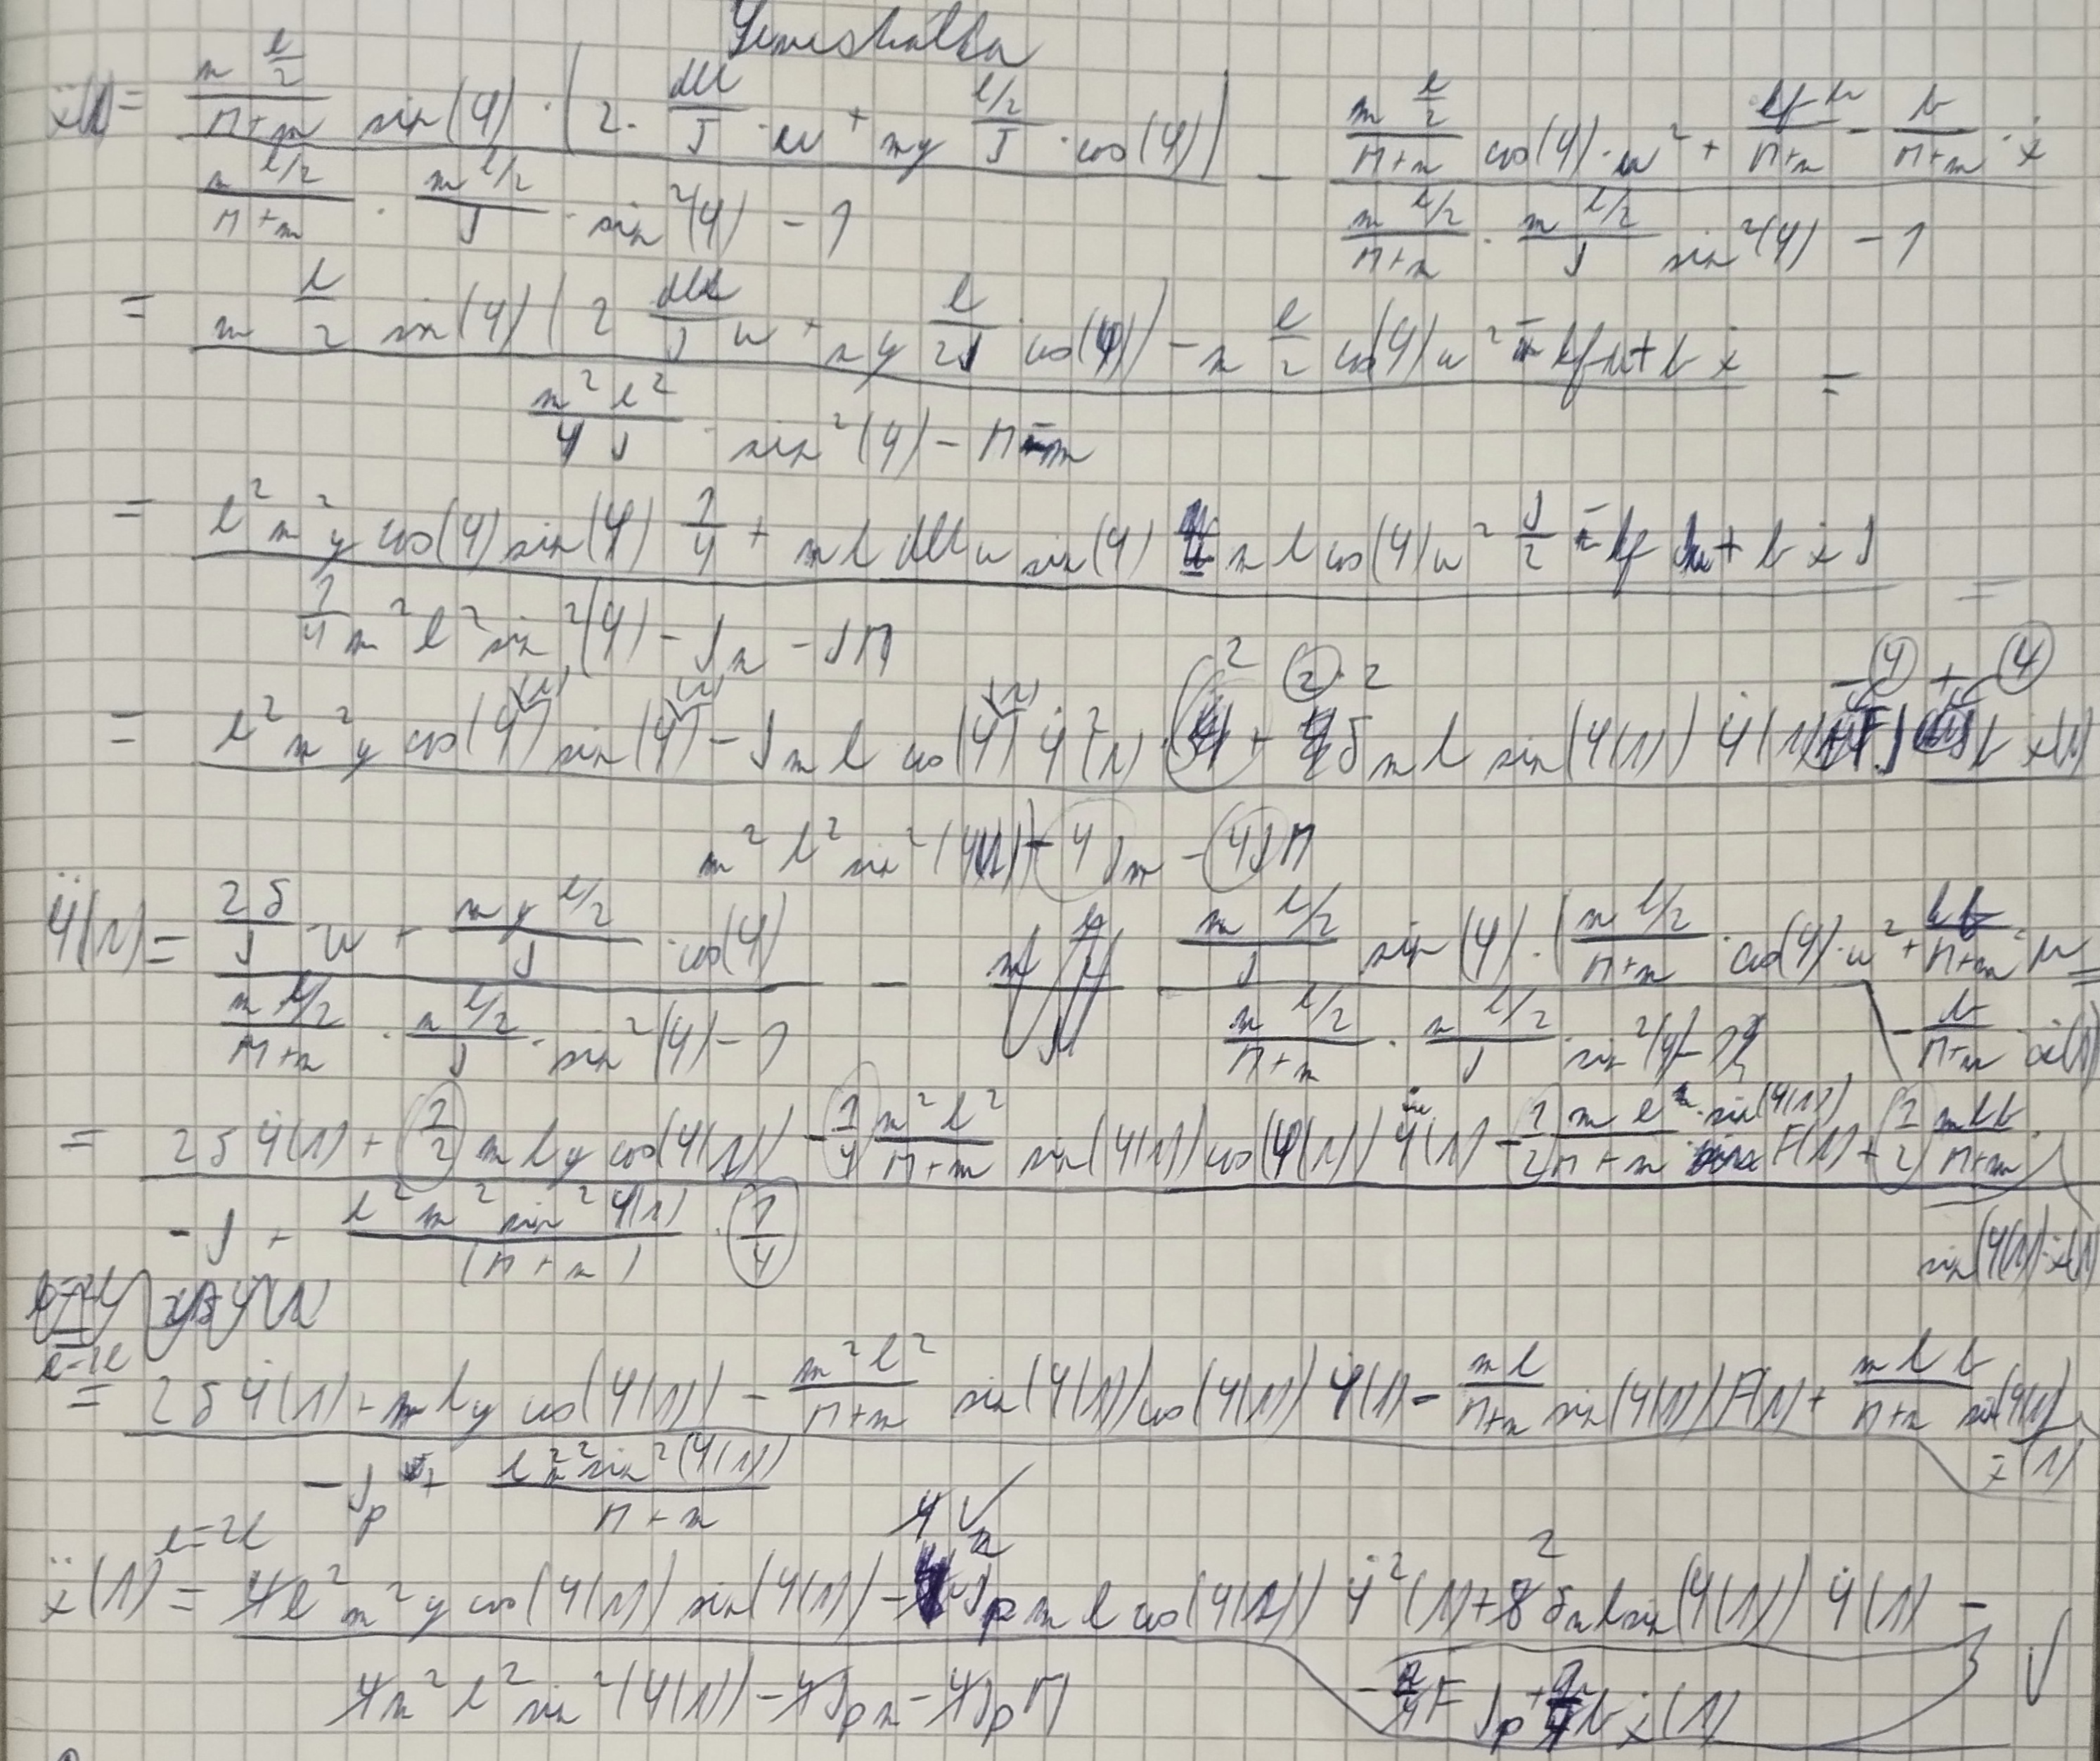
\includegraphics[width=1\textwidth]{img/equation_check.jpg}
  \caption{Kontrola rovnic}\label{fig:equation_check}
\end{figure}

Rovnice vypadají po přepsání stejně, až na to, že v Matlabu je hodnota $l$ všude
vynásobena $2$. Jedná se o chybu ve značení mezi délkou celého kyvadla a
vzdáleností od konce kyvadla po jeho těžiště. Dále budu pokračovat s údaji z
Matlabu. Ještě jsem si všimnul, že v pdf zadání se nachází drobná chyba v
jednotkách pro $J_p$: setrvačnost musí mít jednotku [kg\,m$^2$]. 
 
\subsection{Omezení vstupu a výstupu}
Pro vstupní napětí je v zadaném programu uvedena saturace: vozík bude přijímat
signál v rozsahu $u \in [-10; 10]$.  Dále jsem zjistil hodnotu deadzone - vozík
nereaguje na napětí s hodnotou $\mathrm{abs}(u)\leq0.2$. Test jsem provedl 
postupným zvyšováním napětí na vstupu, dokud se vozík nezačal pohybovat, 
viz obrázek~\ref{fig:Deadzone}.

\begin{figure}[htbp]
  \centering
  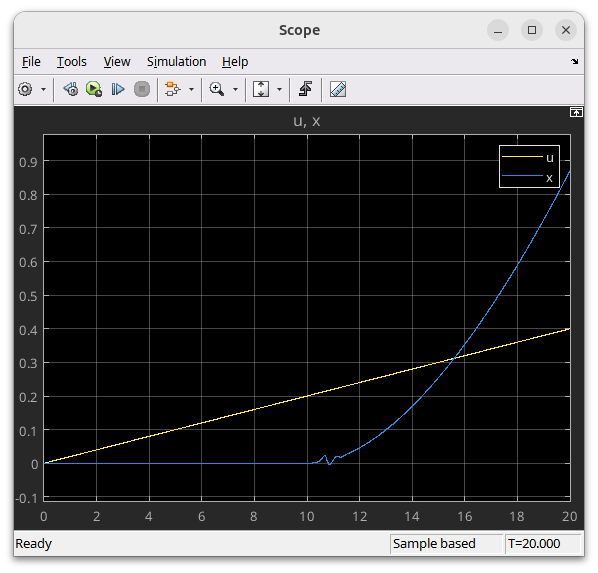
\includegraphics[width=0.8\textwidth]{img/deadzone.png}
  \caption{Zjišťování deadzone}\label{fig:Deadzone}
\end{figure}

\section{Linearizace}
Abych mohl efektivně pracovat s rovnicemi, tak je potřebuji linearizovat v
určitých bodech. Pro účely úlohy potřebuji získat linearizované rovnice kyvadla
pro $\varphi = -90$° (kyvadlo míří kolmo dolů) a pro $\varphi = 90$° (kyvadlo
míří kolmo nahoru). Linearizaci pro dolní a horní polohu provedu pomocí Matlabu
následovně:

\begin{verbatim}
A_sym = jacobian(f, X);
B_sym = jacobian(f, u);

X = [v; y; w; phi]; 
f = [dv; dy; dw; dphi];

X_down = [0; 0; 0; -pi/2];
u_eq = 0;
A_down = double(subs(A_sym, [X; u], [X_down; u_eq]));
B_down = double(subs(B_sym, [X; u], [X_down; u_eq]));

X_up = [0; 0; 0; pi/2];
A_up = double(subs(A_sym, [X; u], [X_up; u_eq]));
B_up = double(subs(B_sym, [X; u], [X_up; u_eq]));
\end{verbatim}

\subsection{Rekce lineárního a nelineárního systému na vstupy}
Systém zapojím podle obrázku~\ref{fig:lin_testing_simulink}. Budu testovat pouze dolní
polohu, horní je nestabilní (viz níže) a kyvadlo by hned spadlo. Na vstup budu
pouštět sinusový signál o různé amplitudě. Mohu pozorovat, že pro slabý vstupní
signál dochází k problémům s deadzonem, viz
obrázky~\ref{fig:lin_testing_deadzone_x} a~\ref{fig:lin_testing_deadzone_phi}.

\begin{figure}[htbp]
  \centering
  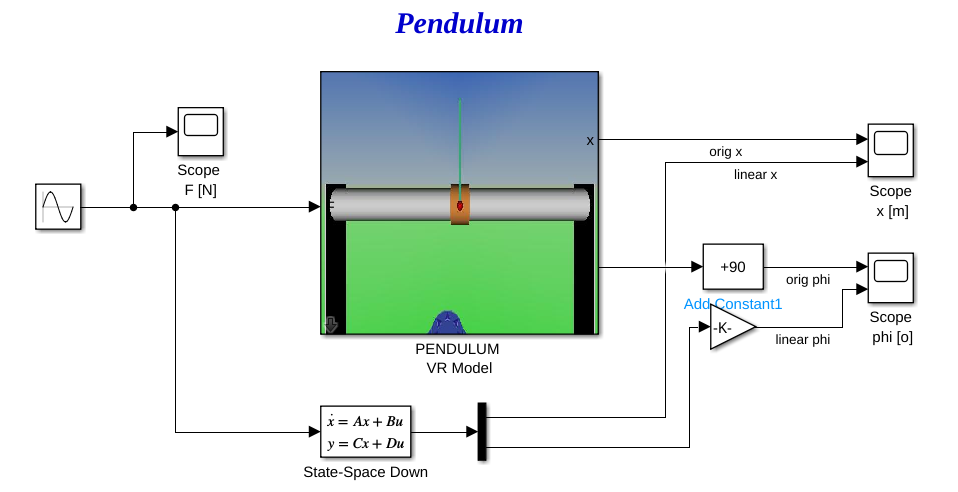
\includegraphics[width=0.8\textwidth]{img/lin_testing_simulink.png}
  \caption{Zapojení v Simulinku pro testování linearizace}\label{fig:lin_testing_simulink}
\end{figure}

\begin{figure}[htbp]
  \centering
  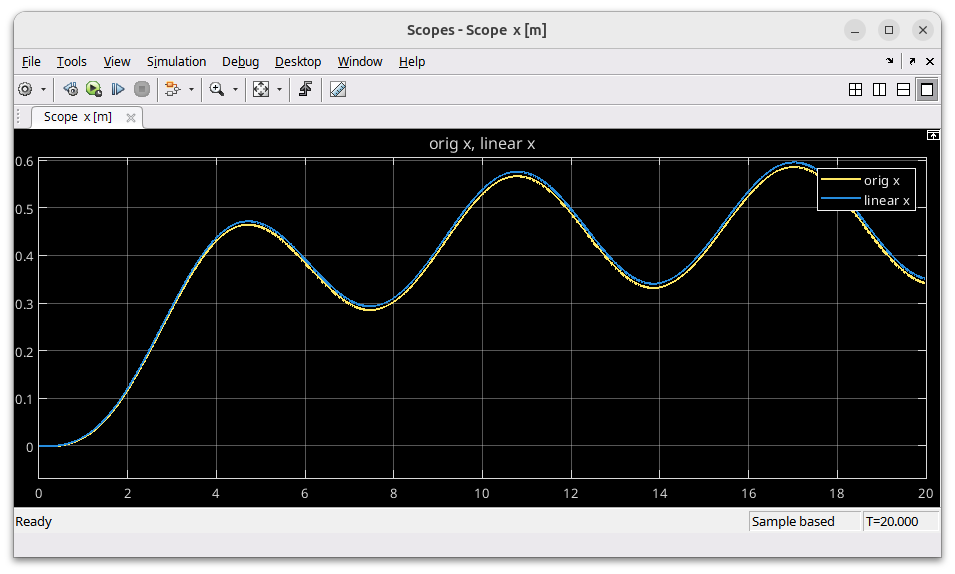
\includegraphics[width=0.8\textwidth]{img/lin_testing_deadzone_x.png}
  \caption{Testování linearizace pro polohu vozíku s amplitudou vstupu 1}\label{fig:lin_testing_deadzone_x}
\end{figure}

\begin{figure}[htbp]
  \centering
  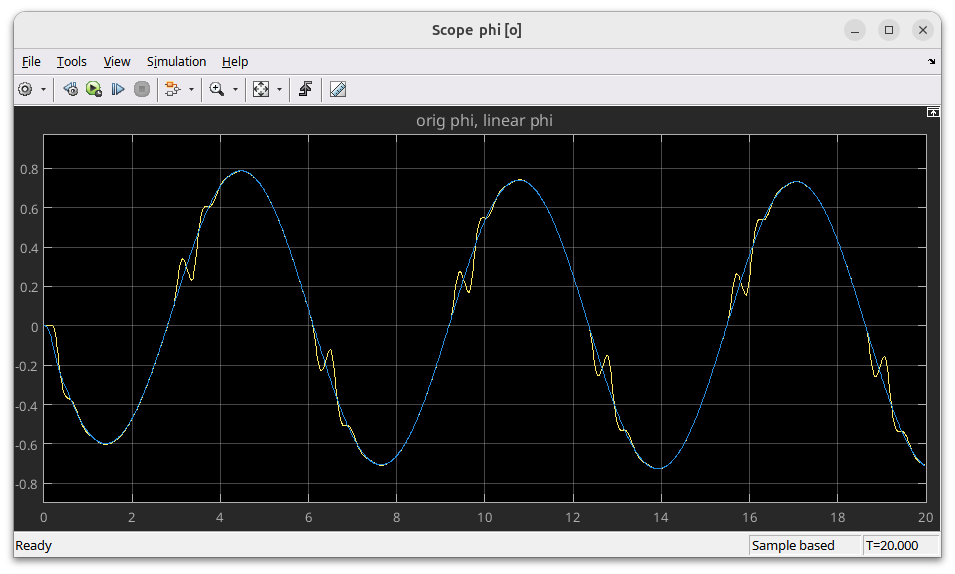
\includegraphics[width=0.8\textwidth]{img/lin_testing_deadzone_phi.png}
  \caption{Testování linearizace pro úhel kyvadla s amplitudou vstupu 1}\label{fig:lin_testing_deadzone_phi}
\end{figure}

Pro vyšší amplitudy (zvolil jsem 10) už dochází k nepřesnosti linearizace ve
špičkách, jak ukazuje obrázek~\ref{fig:lin_testing_error}. Pro signály s větší 
amplitudou by docházelo k chybě kvůli saturaci.

\begin{figure}[htbp]
  \centering
  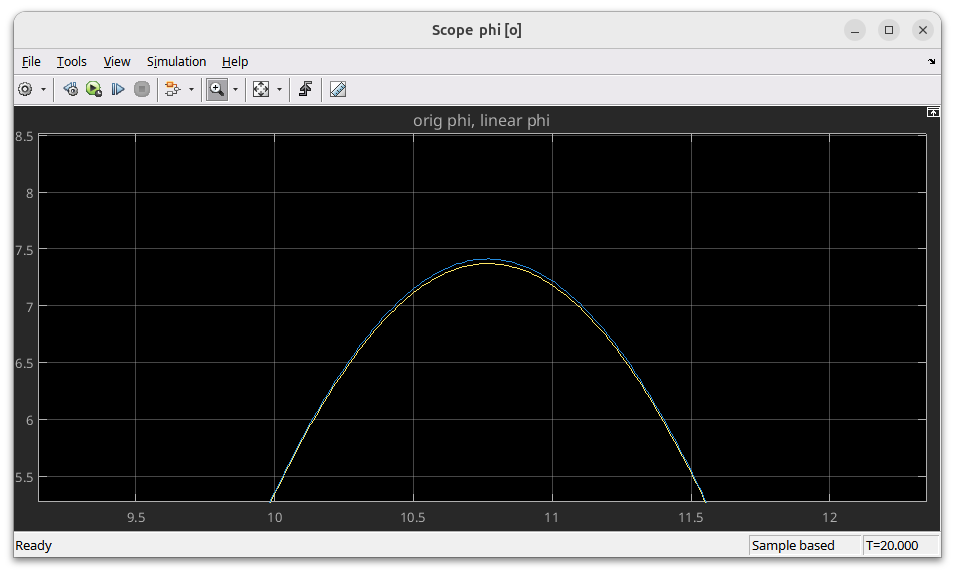
\includegraphics[width=0.8\textwidth]{img/lin_testing_error.png}
  \caption{Testování linearizace pro úhel kyvadla s amplitudou vstupu 10}\label{fig:lin_testing_error}
\end{figure}

\section{Vlastnosti systému - otevřené smyčky}
\subsection{Póly}
Zajímají mě póly a nuly systému pro obě polohy - mohu si tak například potvrdit
stabilitu, respektive nestabilitu dolní, respektive horní polohy, popřípadě je
využít v při pozdějším návrhu regulátorů. Číselné hodnoty pólů mohu dostat
například pomocí příkazu \texttt{eig(A\_down)} zavolaného na matici A. Ovšem
vhodnější bude grafické znázornění, do kterého vložím stavový popis systému:

\begin{verbatim}
C = [0 1 0 0;
     0 0 0 1];
D = [0; 0];

sys_ss_down =  ss(A_down, B_down, C, D);
sys_ss_up =  ss(A_up, B_up, C, D);

pzmap(sys_ss_down);
pzmap(sys_ss_up);
\end{verbatim}

Matice C a D jsou v tomto stavu, protože mě zajímá poloha vozíku a úhel kyvadla, 
tedy $2.$ a $4.$ složka systému. Póly pro dolní polohu jsou na
obrázku~\ref{fig:poles_down} a pro horní polohu na~\ref{fig:poles_up}.

\begin{figure}[htbp]
  \centering
  \begin{minipage}{0.49\textwidth}
    \centering
    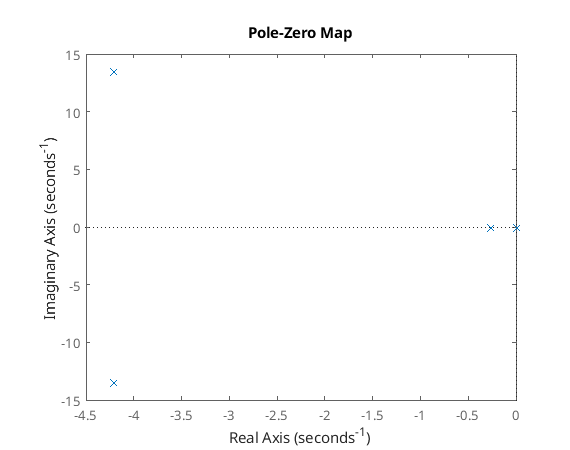
\includegraphics[width=\linewidth]{img/poles_down.png}
    \caption{Póly pro dolní polohu}\label{fig:poles_down}
  \end{minipage}\hfill
  \begin{minipage}{0.49\textwidth}
    \centering
    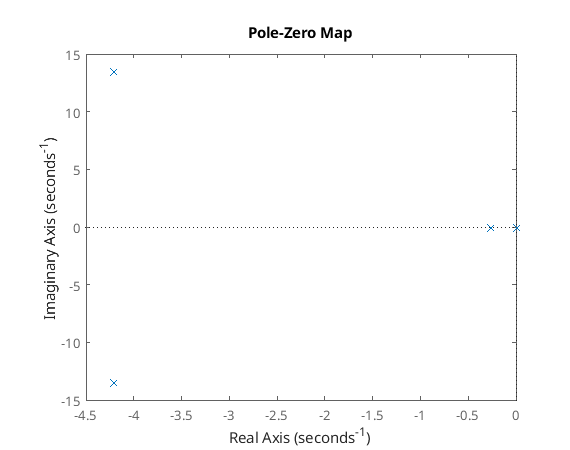
\includegraphics[width=\linewidth]{img/poles_up.png}
    \caption{Póly pro horní polohu}\label{fig:poles_up}
  \end{minipage}
\end{figure}

Pro dolní polohu mám následující póly:

\begin{itemize}
  \item $0$...integrátor - vozík nemá tendenci se vracet
  \item $-0.27$...reálný pomalý pól - tření vozíku
  \item $-4.21 \pm 13.52 i$...komplexně sdružená dvojice - kyvadlo kmitá
  frekvencí $13.52 \mathrm{rad}\cdot\mathrm{s}^{-1}$ a $-4.21$ je tlumení
  třením kyvadla.
\end{itemize}

A pro horní polohu mám následující póly:

\begin{itemize}
  \item $0$...integrátor - vozík nemá tendenci se vracet
  \item $-0.27$...reálný pomalý pól - tření vozíku
  \item $18.98$...rychlý reálný pól - prudké tlumení kyvadla
  \item $10.56$...nestabilní pól - gravitace, která shazuje kyvadlo dolů
\end{itemize}

\subsection{Přenos}
Systém má jeden vstup, ale dva výstupy (SIMO). Neexistují frekvence na vstupu,
které by zablokovaly oba výstupy najednou. Proto nevidím žádné nuly celého
systému.  Ale z jednotlivých přenosů napětí $\rightarrow$ poloha a napětí
$\rightarrow$ úhel bych nuly získal.

Přenosové funkce pro dolní polohu:
\begin{align*}
    G_{down, x}(s) &= \frac{0.18 s^2 + 1.07 s + 25.86}{s(s^3 + 8.69 s^2 + 202.7 s + 54.31)} \\
    G_{down, \phi}(s) &= \frac{-2.64 s}{s^3 + 8.69 s^2 + 202.7 s + 54.31}
\end{align*}

Přenosové funkce pro horní polohu:
\begin{align*}
    G_{up, x}(s) &= \frac{0.18 s^2 + 1.07 s - 25.86}{s(s^3 + 8.69 s^2 - 198.2 s - 54.31)} \\
    G_{up, \phi}(s) &= \frac{2.64 s}{s^3 + 8.69 s^2 - 198.2 s - 54.31}
\end{align*}

Z přenosů mohu zjistit nějaké zajímavé vlastnosti. Například oba přenosy pro
polohu mají pól v $0$, tedy integrátor. Nula v počátku pro oba přenosy pro úhel
znamená, že statické zesílení těchto přenosů je rovno nule - při jízdě vozíku
konstantní rychlostí by kyvadlo viselo dolů, popřípadě nahoru.

Nuly pro přenos polohy v dolní poloze kyvadla vycházejí na $s = -3.05 \pm 11.7i$. Dostávám tak 
antirezonanční frekvenci - pokud bych zanedbal tření, tak se bude kyvadlo kývat, ale 
vozík se nepohne.

Pro horní polohu a její přenos pro polohu dostávám následují nuly: $-15.5$, $9.41$. Nula v 
pravé polorovině mi dává neminimální fázi - abych pohnul s vozíkem a kyvadlo mi nespadlo, 
musím nejdřív pohnout na opačnou stranu.

\section{Řízení polohy vozíku pomocí PID regulátoru}
Jako první úlohu jsem si zvolil řízení polohy vozíku - dostanu zadaný bod na ose
x a cílem je, aby na něj vozík dojel. Během této fáze budu zcela ignorovat pohyb
kyvadla.

\subsection{Zapojení v Simulinku}
Pro zprovoznění simulace jsem nejdříve zapojil schéma v Simulinku
\ref{fig:Simulink_pos_PID}. Linearizaci provádím přes blok \texttt{State-Space},
do kterého jsem dal matice \texttt{A\_down}, \texttt{B\_down}, \texttt{C} a
\texttt{D}.

\begin{figure}[htbp]
  \centering
  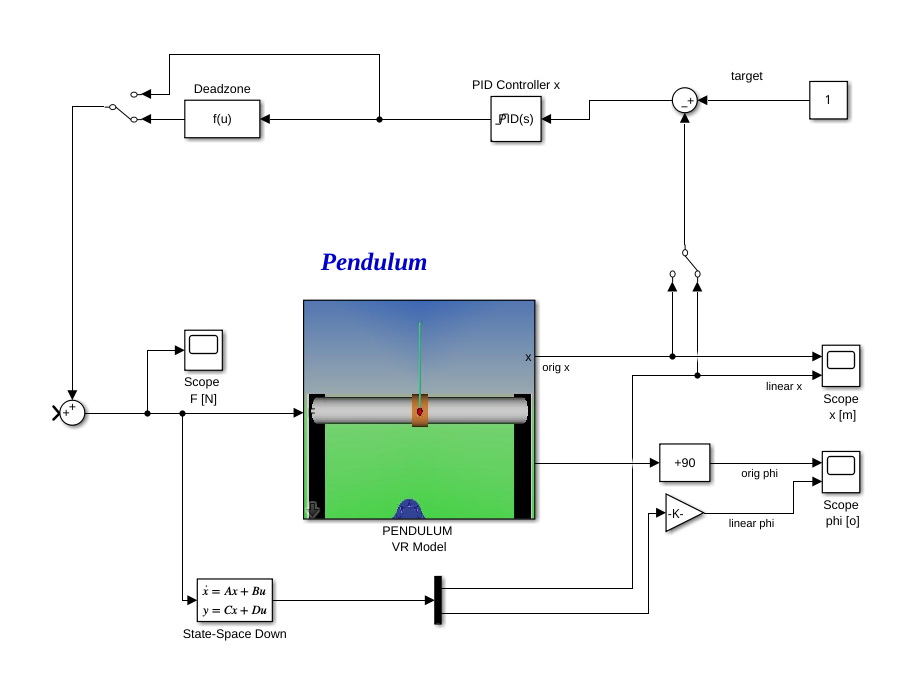
\includegraphics[width=0.8\textwidth]{img/simulink_pos_PID.png}
  \caption{Zapojení v Simulinku pro regulátor polohy vozíku}\label{fig:Simulink_pos_PID}
\end{figure}

Z linearizovaného modelu vedu signál do Scope pro polohu a pro úhel (rozděluji
ho pomocí bloku Demux), úhel musím převést na stupně.

Ve zpětné vazbě mám regulátor, do kterého později dosadím získané hodnoty.
Regulátor sám o sobě obsahuje omezení na saturaci a implementaci řešení
wind-upu (zvolil jsem metodu clamping - když signál přesahuje hodnotu saturace,
tak dále nenačítám I složku regulátoru). Následuje blok, který signál ořízne,
pokud se nachází v deadzone. Po přidání těchto bloků jsou nelineární i lineární
signál během řízení v dolní poloze téměř shodné,
viz~\ref{fig:Without_sat_and_deadzone_in}
a~\ref{fig:Without_sat_and_deadzone_out}.

\begin{figure}[htbp]
  \centering
  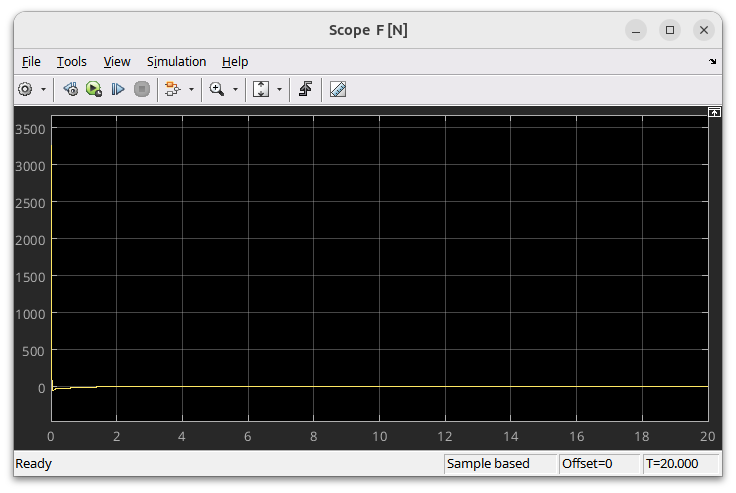
\includegraphics[width=0.8\textwidth]{img/without_sat_and_deadzone_in.png}
  \caption{Zapojení bez saturace a deadzone - vstup}\label{fig:Without_sat_and_deadzone_in}
\end{figure}

\begin{figure}[htbp]
  \centering
  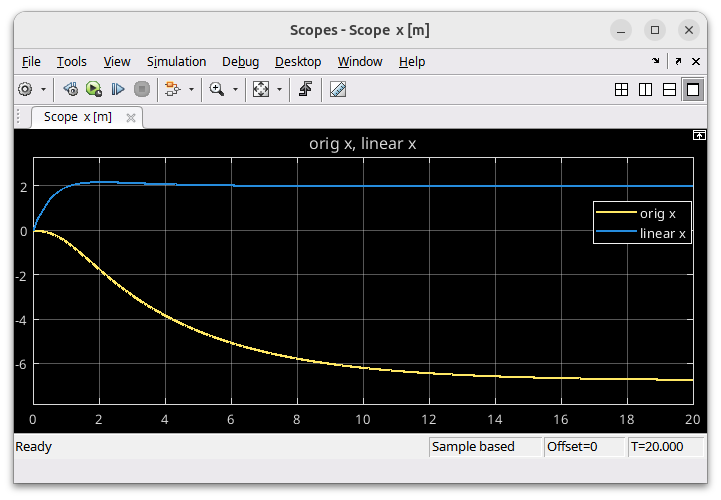
\includegraphics[width=0.8\textwidth]{img/without_sat_and_deadzone_out.png}
  \caption{Zapojení bez saturace a deadzone - výstup}\label{fig:Without_sat_and_deadzone_out}
\end{figure}

\subsection{P regulátor}
Nejdříve jsem vyzkoušel řízení pomocí samotného P regulátoru, které ovšem vedlo
na mnoho problémů. Při vysoké hodnotě koeficientu Kp docházelo k velkému
překmitu a následnému rozkmitání, kvůli kterému se kyvadlo nechtělo ustálit na
cílové hodnotě - výsledky jsou na obrázku~\ref{fig:P_pos_overshoot}.

\begin{figure}[htbp]
  \centering
  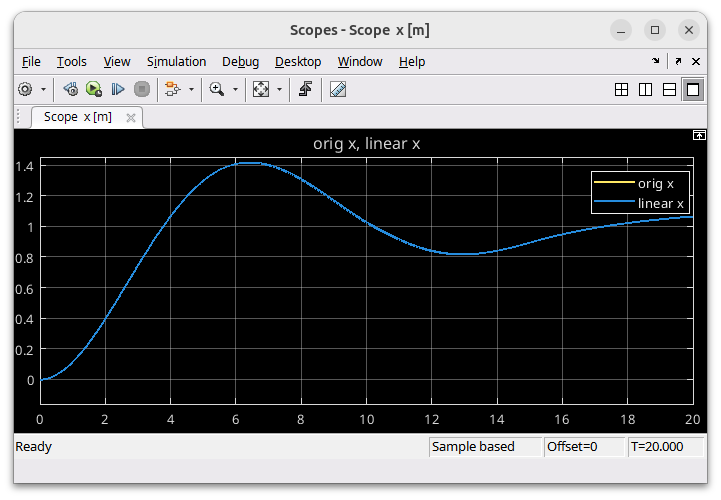
\includegraphics[width=0.8\textwidth]{img/P_pos_overshoot.png}
  \caption{Překmit P regulátoru}\label{fig:P_pos_overshoot}
\end{figure}

I pro výsledky s řádně odladěnou hodnotou $K_p = 1.1$ (viz
obr.~\ref{fig:rltool_p_pos}) nastával klasický problém u P regulátoru, a to že
se kyvadlo neustálí na cílové hodnotě, jako na
obrázku~\ref{fig:P_pos_inf_error}. Tento jev je navíc výrazně podpořen existencí
pásma necitlivosti, které dělá tento problém neřešitelným. Pro P regulátor mi z
Bodeho a Nyquistova grafu na obrázku~\ref{fig:bode_nyquist_p} vychází 
$\mathrm{GM} = \infty$, $\mathrm{PM} = 39.2^\circ$.

\begin{figure}[htbp]
  \centering
  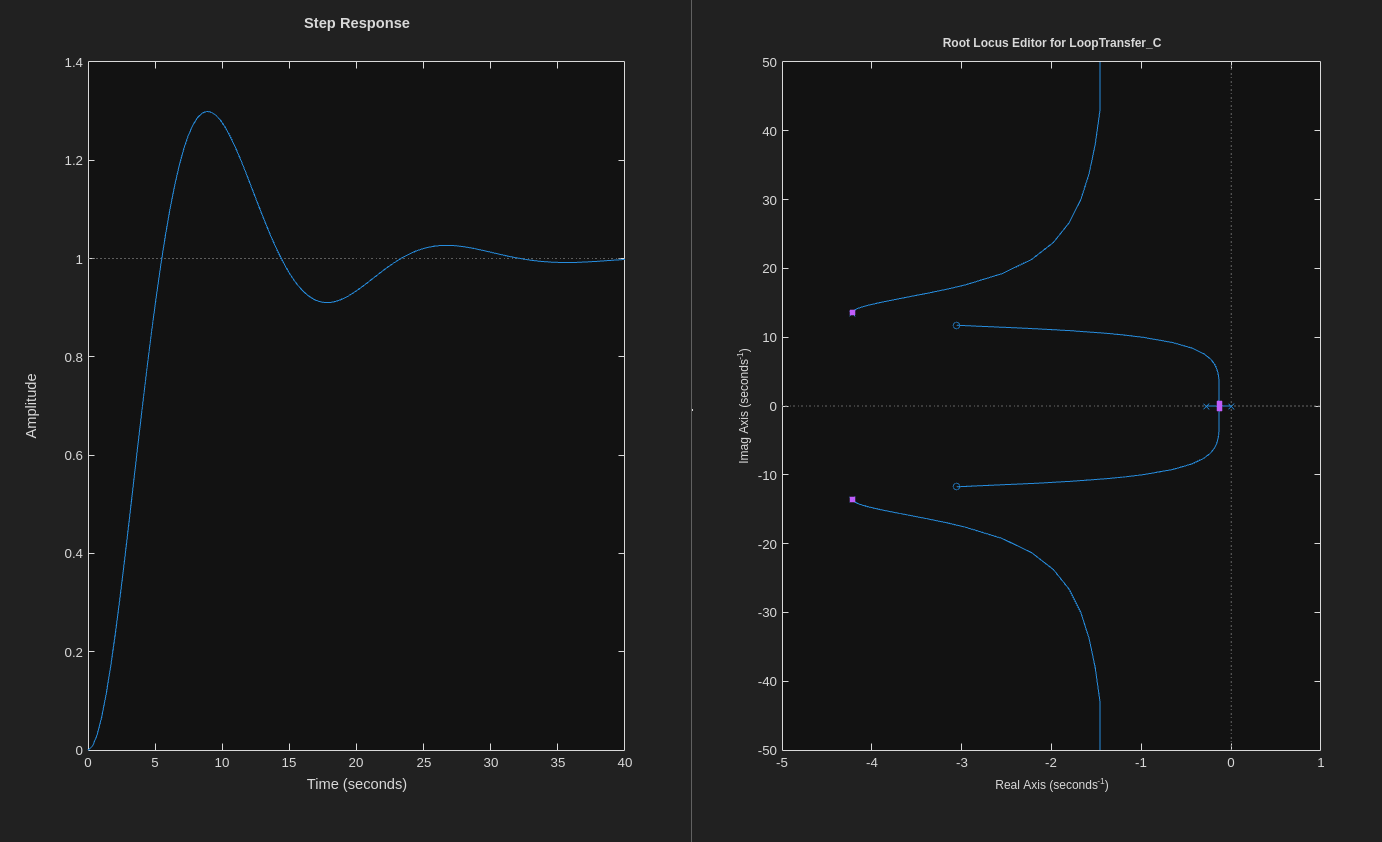
\includegraphics[width=0.8\textwidth]{img/rltool_p_pos.png}
  \caption{Root locus pro P regulátor}\label{fig:rltool_p_pos}
\end{figure}

\begin{figure}[htbp]
  \centering
  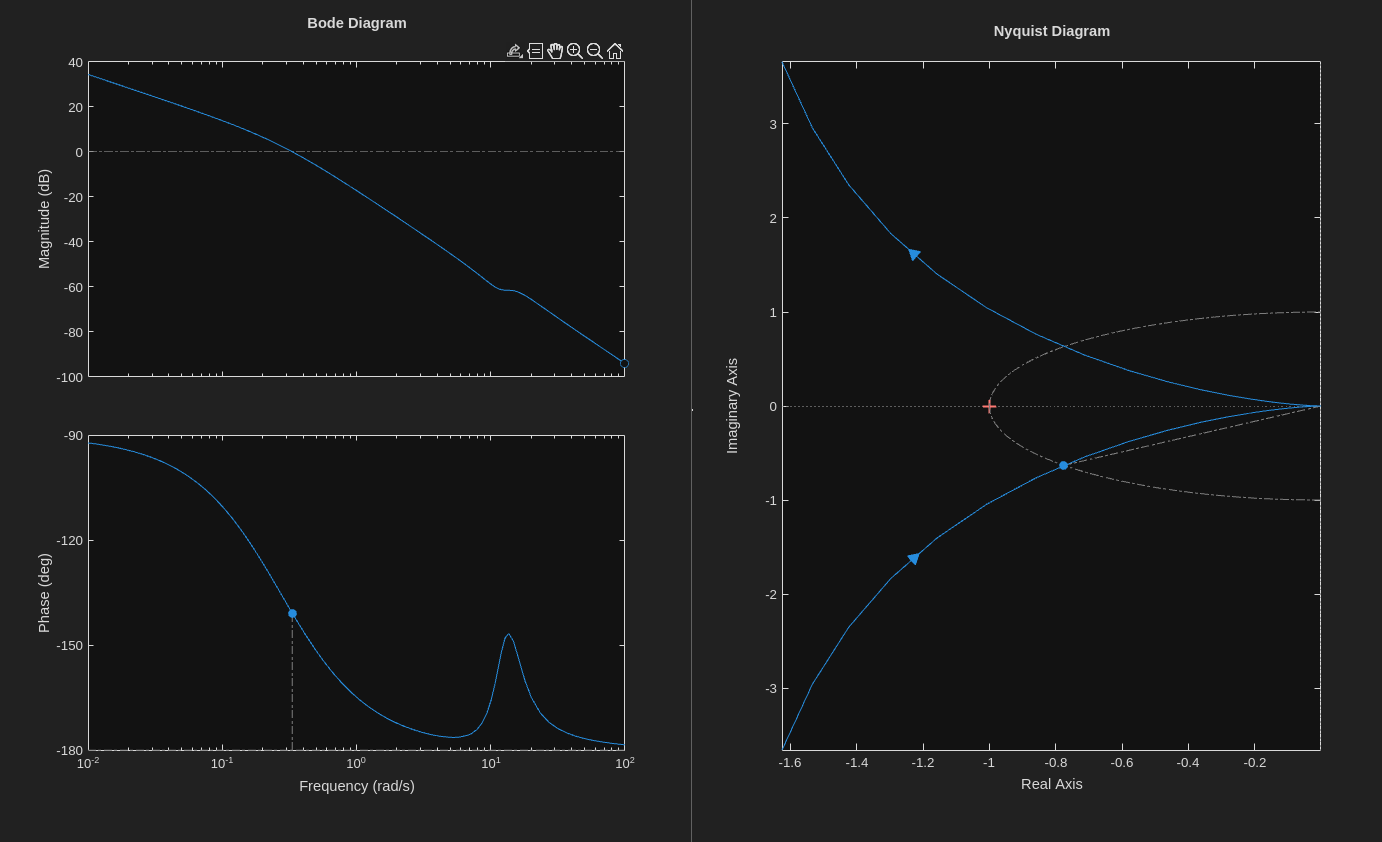
\includegraphics[width=0.8\textwidth]{img/bode_nyquist_p.png}
  \caption{Bodeho a Nyquistův graf pro P regulátor}\label{fig:bode_nyquist_p}
\end{figure}

\begin{figure}[htbp]
  \centering
  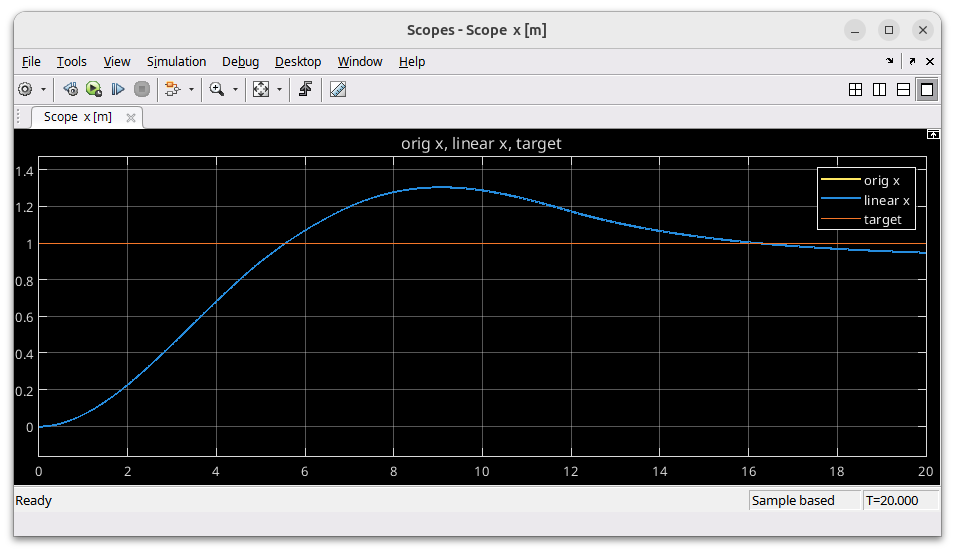
\includegraphics[width=0.8\textwidth]{img/P_pos_inf_error.png}
  \caption{Ustálení na špatné hodnotě P regulátoru}\label{fig:P_pos_inf_error}
\end{figure}

\subsection{PD regulátor}
Přidáním D složky jsem schopen omezit překmit téměř na minimum, ale stále se
nezbavím odchylky v nekonečnu, viz obr.~\ref{fig:PD_pos}. Regulátor jsem odladil
v programu \texttt{rltool}~\ref{fig:rltool_pd_pos} na hodnoty $K_p = 6.28$, $K_d
= 14.5$. Z obrázku~\ref{fig:bode_nyquist_pd} mám $\mathrm{GM} = \infty$,
$\mathrm{PM} = 85.2^\circ$.

\begin{figure}[htbp]
  \centering
  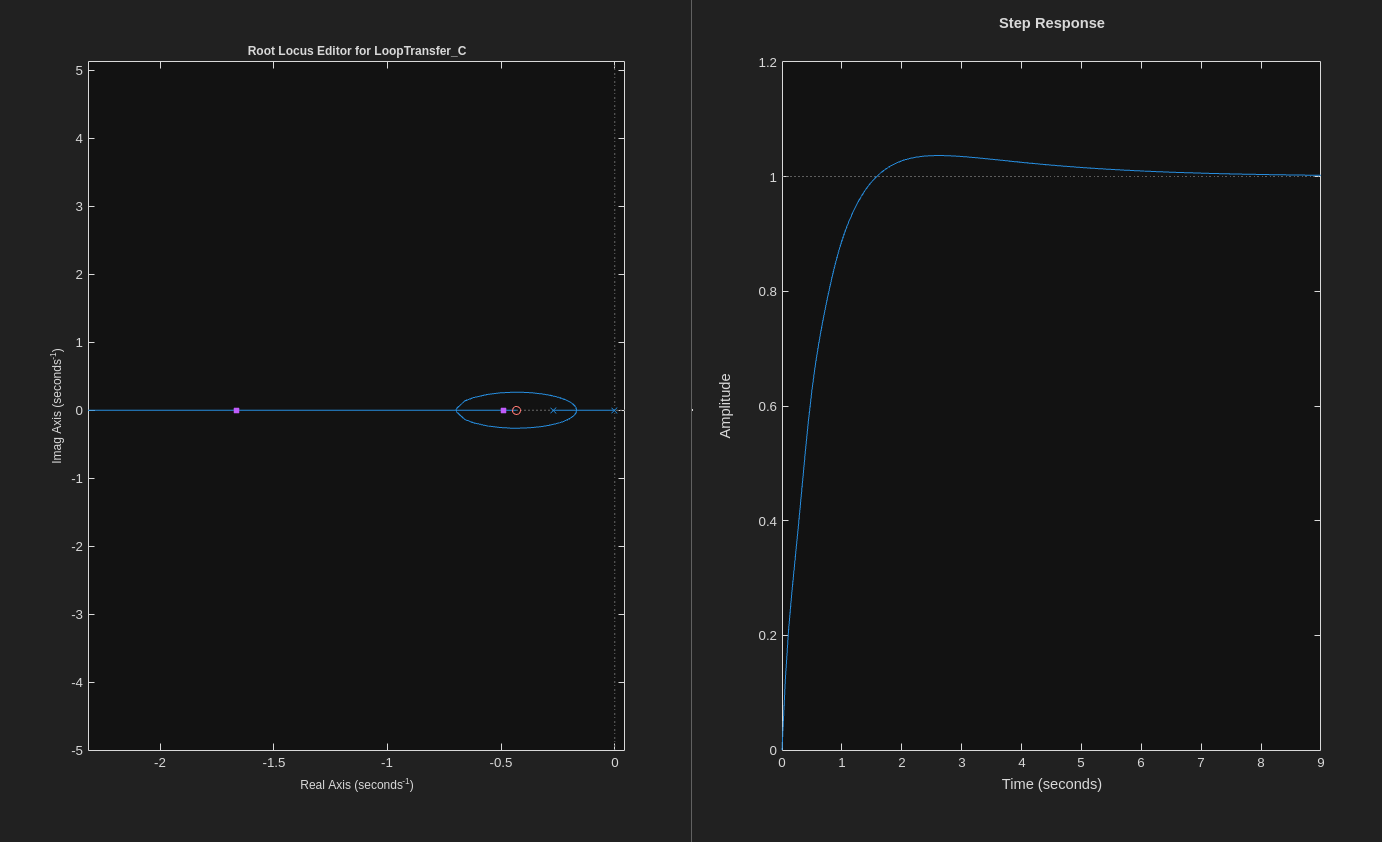
\includegraphics[width=0.8\textwidth]{img/rltool_pd_pos.png}
  \caption{Root locus pro PD regulátor}\label{fig:rltool_pd_pos}
\end{figure}

\begin{figure}[htbp]
  \centering
  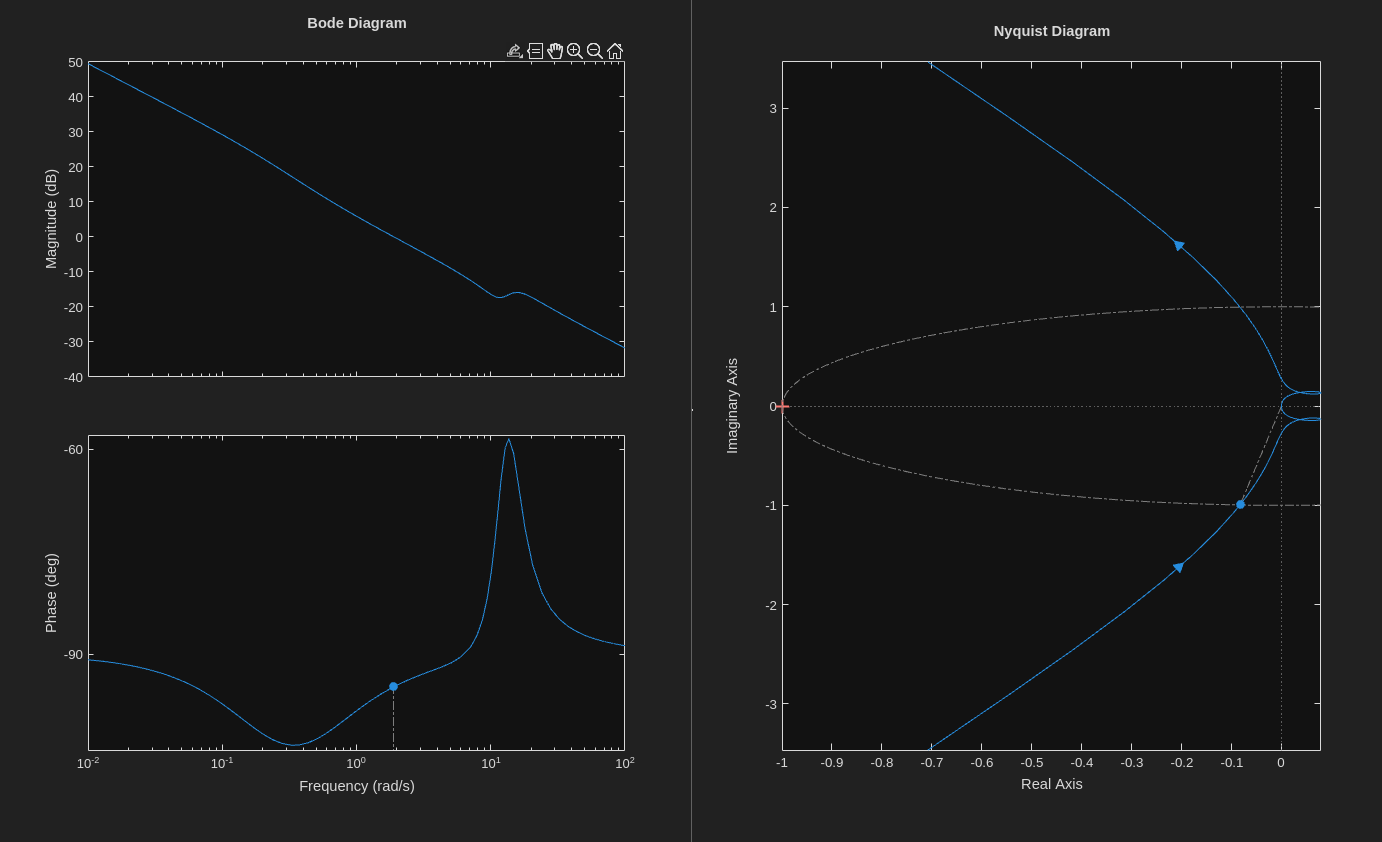
\includegraphics[width=0.8\textwidth]{img/bode_nyquist_pd.png}
  \caption{Bodeho a Nyquistův graf pro PD regulátor}\label{fig:bode_nyquist_pd}
\end{figure}

\begin{figure}[htbp]
  \centering
  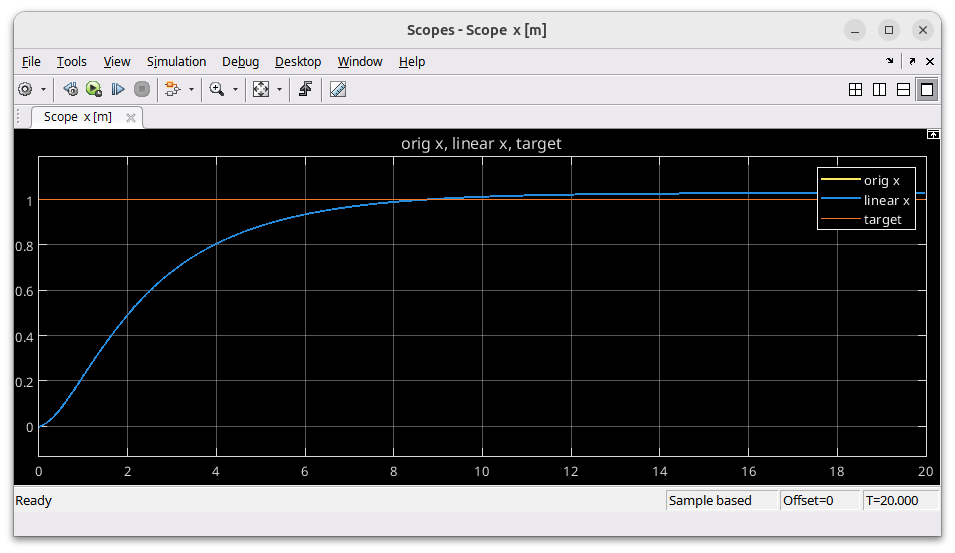
\includegraphics[width=0.8\textwidth]{img/PD_pos.png}
  \caption{Řízení polohy vozíku s PD regulátorem}\label{fig:PD_pos}
\end{figure}


Z výše zmíněných důvodů je nutné implementovat PID regulátor.

\subsection{PID regulátor}
PID už zvládá vozík regulovat dostatečně dobře. Hodnoty jsem odladil pomocí
programu \texttt{rltool}~\ref{fig:rltool_pid_pos} a dosadil je do schématu
Simulinku.  Výsledná regulace na polohu $x=1$ (na obrázku~\ref{fig:PID_pos}) má
překmit menší než $15 \%$ a dobu ustálení na $90 \%$ reference za $11
\mathrm{s}$. Podle grafů Bodeho a Nyquista na obrázku~\ref{fig:bode_nyquist_pid} znám 
$\mathrm{GM} = \infty$, $\mathrm{PM} = 80.5^\circ$.

\begin{figure}[htbp]
  \centering
  
\includegraphics[width=0.8\textwidth]{img/rltool_pid_pos.png}
  \caption{Root locus pro PID regulátor}\label{fig:rltool_pid_pos}
\end{figure}

\begin{figure}[htbp]
  \centering
  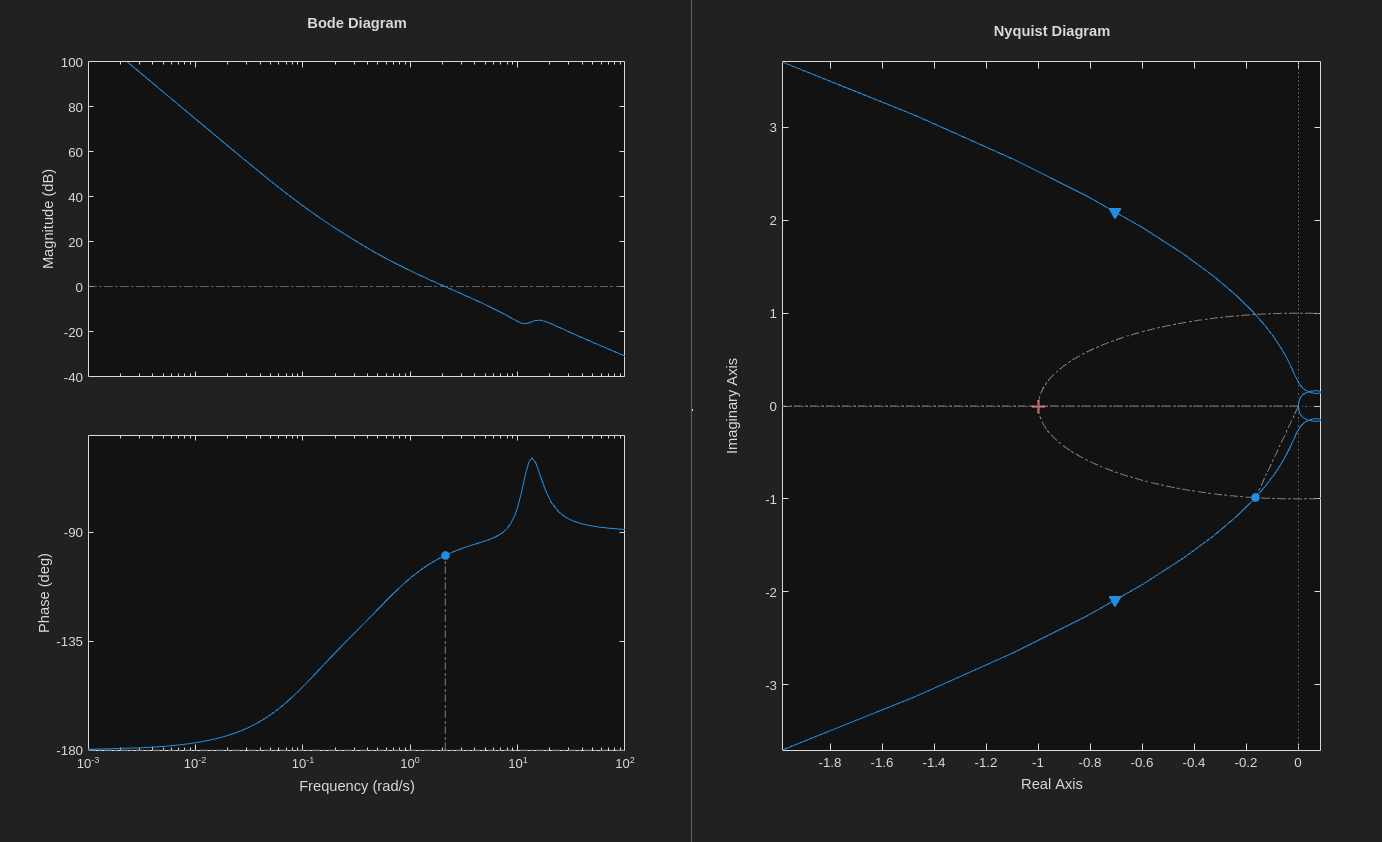
\includegraphics[width=0.8\textwidth]{img/bode_nyquist_pid.png}
  \caption{Bodeho a Nyquistův graf}\label{fig:bode_nyquist_pid}
\end{figure}

\begin{figure}[htbp]
  \centering
  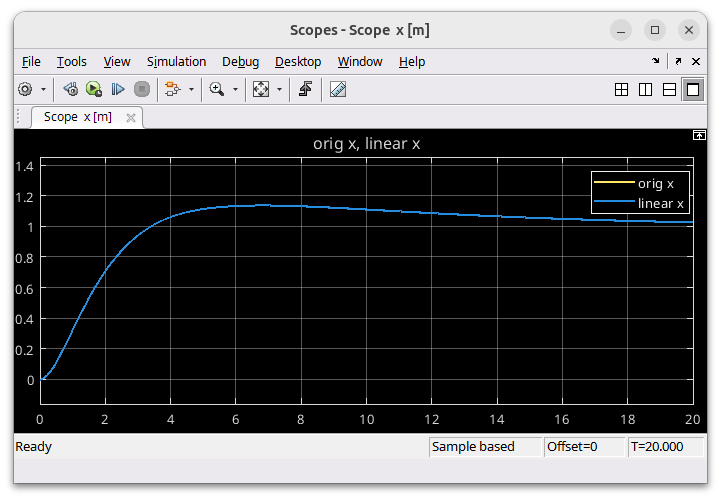
\includegraphics[width=0.8\textwidth]{img/PID_pos.png}
  \caption{Regulace vozíku na polohu $x=1$}\label{fig:PID_pos}
\end{figure}

\subsection{Model reference}
Tato metoda se neprobírala na přednáškách, ovšem po času stráveném na
implementaci jsem se rozhodl ji zde ponechat.

Zatím jsem měl jako referenci nastavenou konstantu, jednalo se vlastně o
jednotkový skok. Pro lepší řízení mohu ovšem referenci postupně načítat (pomocí
přenosu) a tím se vyhnout zbytečně velkému překmitu. Za blok target připojím
přenos druhého stupně, jehož hodnoty odladím a dostanu tak efektivnější řízení
vozíku. Pro přenos $\frac{1}{0.05s^2 + s + 1}$ dostávám překmit $5 \%$ a v
rozmezí $\pm 5 \%$ od cílové hodnoty bude vozík za $2.6 \mathrm{s}$. Graf je na
obrázku~\ref{fig:reference_model}. 

\begin{figure}[htbp]
  \centering
  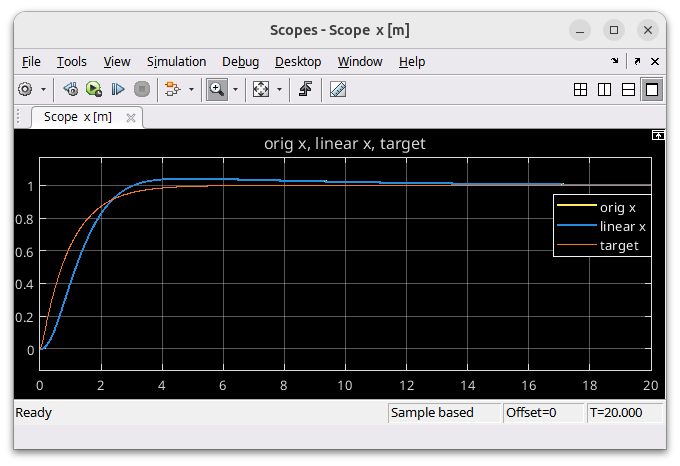
\includegraphics[width=0.8\textwidth]{img/reference_model.png}
  \caption{Regulace vozíku s modelem reference}\label{fig:reference_model}
\end{figure}

Tímto způsobem, s přenosem $\frac{1}{0.03s^2 + 2.8s + 1}$, jsem dosáhl i řízení
polohy vozíku s překmitem méně než $1 \%$, do intervalu $1 \%$ od cílové hodnoty
se vozík dostane za $9 \mathrm{s}$.

\section{Řízení polohy vozíku pomocí PID regulátoru s přidaným tlumením kmitů}
Řízení polohy vozíku už funguje, teď se budu snažit, abych utlumil kmitání
kyvadla během pohybu vozíku.

\subsection{Tlumení kmitů pomocí D regulátoru}
Následujícím cílem mé práce je utlumit kmitání kyvadla během posunu vozíku. 
Budu testovat PD a D regulátor. Do simulinku si přidám blok regulátoru, do
kterého vede jako vstup úhel kyvadla. Jedná se o tlumení, takže výsledná
hodnota pro regulaci musí být vždy záporná. Hodnoty regulátoru budu chtít
odladit pomocí programu \texttt{rltool} (vkládám systém se záporným znaménkem),
pro D regulátor umístím jednu nulu do bodu 0 a budu hýbat s póly, dokud nezískám
optimální regulátor na obrázku~\ref{fig:rltool_phi}. Z Bodeho a Nyquistova grafu 
na obrázku~\ref{fig:bode_nyquist_phi} vidím, že $\mathrm{GM} = \infty$. $0 \mathrm{dB}$ 
protínám ve dvou bodech s $\mathrm{PM} = 114^\circ$ a $116^\circ$.

\begin{figure}[htbp]
  \centering
  
\includegraphics[width=0.8\textwidth]{img/rltool_phi.png}
  \caption{Hledání parametrů D regulátoru pomocí rltool}\label{fig:rltool_phi}
\end{figure}

\begin{figure}[htbp]
  \centering
  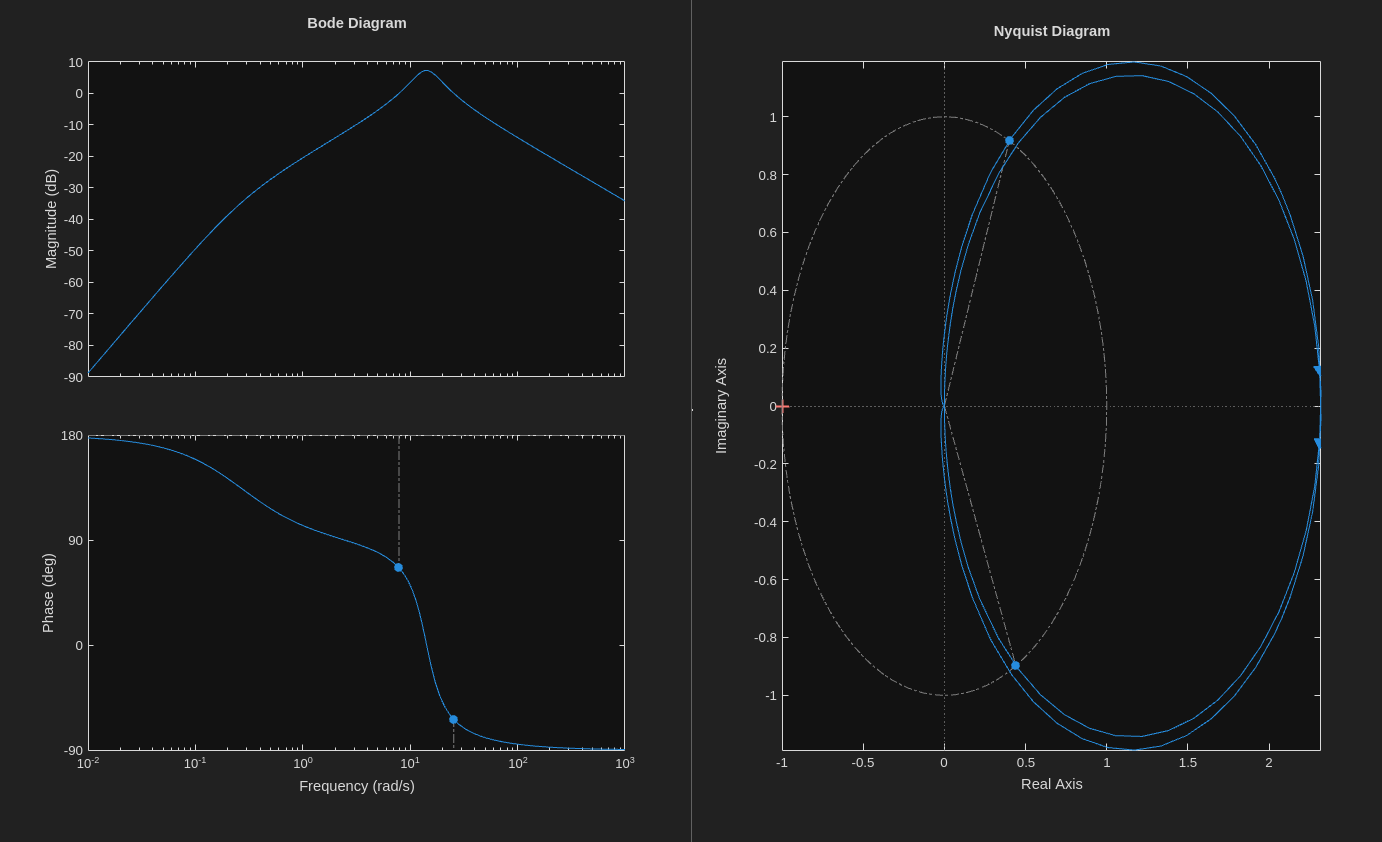
\includegraphics[width=0.8\textwidth]{img/bode_nyquist_phi.png}
  \caption{Bodeho a Nyquistův graf pro úhel kyvadla}\label{fig:bode_nyquist_phi}
\end{figure}

Hodnotu jsem odladil na $k_d = 7.41$. Regulátorem dojde k úplnému utlumení
malých kmitů, tzv. při přesunu vozíku vykoná kyvadlo pouze dva kmity. Zlepšení
oproti původnímu stavu~\ref{fig:oscillation_without} je vidět na
obrázku~\ref{fig:oscillation_with}.

\begin{figure}[htbp]
  \centering
  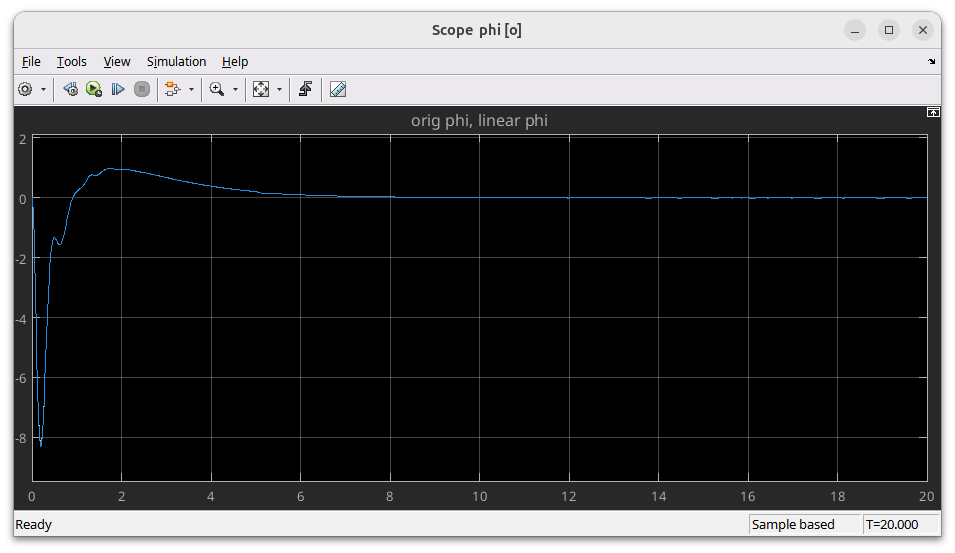
\includegraphics[width=0.8\textwidth]{img/oscillation_without_regulator.png}
  \caption{Kmitání bez regulátoru}\label{fig:oscillation_without}
\end{figure}

\begin{figure}[htbp]
  \centering
  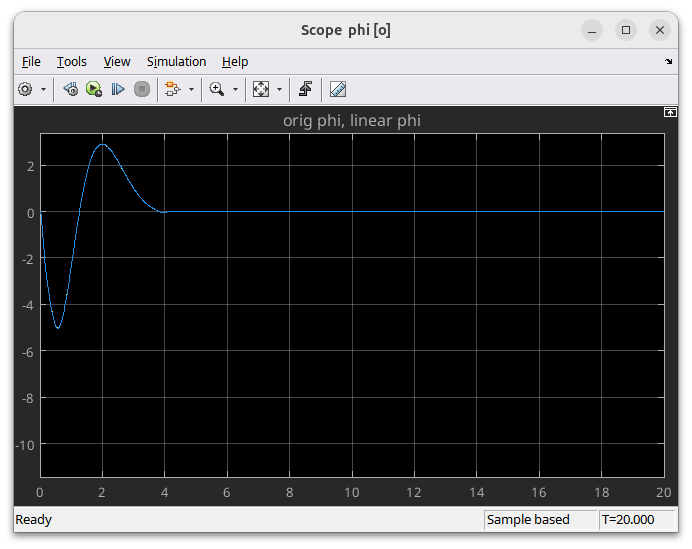
\includegraphics[width=0.8\textwidth]{img/oscillation_with_regulator.png}
  \caption{Kmitání s regulátorem}\label{fig:oscillation_with}
\end{figure}

Přidáním P regulátoru bych sice dosáhl zmenšení prvního kmitu o $\sim 20 \%$, ale
jinak PD regulátor nepřináší žádné výrazné zlepšení, proto ho nebudu
implementovat. Vyvíjím tak totiž zbytečně velkou sílu na vozík.

\subsection{Posicast}
Dále jsem implementoval feedforward řízení posicast. Pomocí funkce
\texttt{damp()} v Matlabu jsem si našel tlumení a frekvenci komplexně sdružených
pólů: $\omega_n = 14.2 \mathrm{rad}\cdot\mathrm{s}^{-1}$ a $\zeta = 0.297$.
Dosadil jsem do vzorců $\tau = \frac{\pi}{\omega_n\sqrt{1-\zeta^2}} =
0.2317\mathrm{s}$ a $\Phi = \frac{1}{1 + e^{-\tau\zeta\omega_n}}=0.7265$.
Posicast rozdělí referenční signál na dva skoky, čímž vyruší kmitání kyvadla ve
výsledné pozici. Pro implementaci a výsledky posicastu viz
obrázky~\ref{fig:posicast_simulink}~\ref{fig:posicast_x}~\ref{fig:posicast_phi}.

\begin{figure}[htbp]
  \centering
  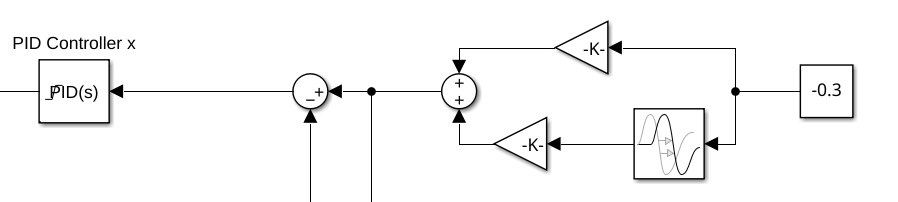
\includegraphics[width=0.8\textwidth]{img/posicast_simulink.png}
  \caption{Implementace posicastu v Simulinku}\label{fig:posicast_simulink}
\end{figure}

\begin{figure}[htbp]
  \centering
  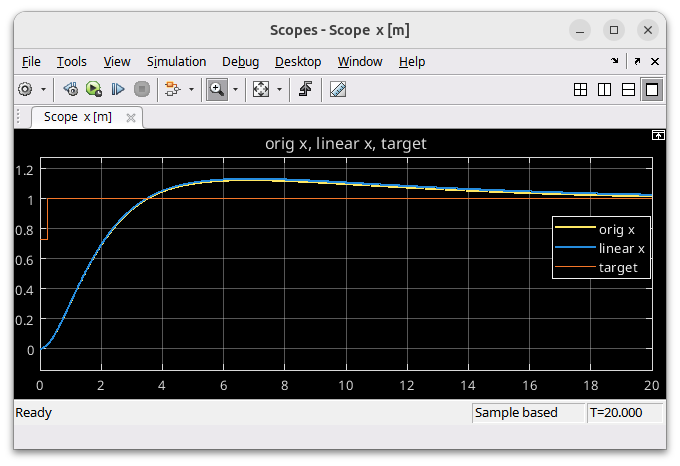
\includegraphics[width=0.8\textwidth]{img/posicast_x.png}
  \caption{Poloha vozíku s poisicastem}\label{fig:posicast_x}
\end{figure}

\begin{figure}[htbp]
  \centering
  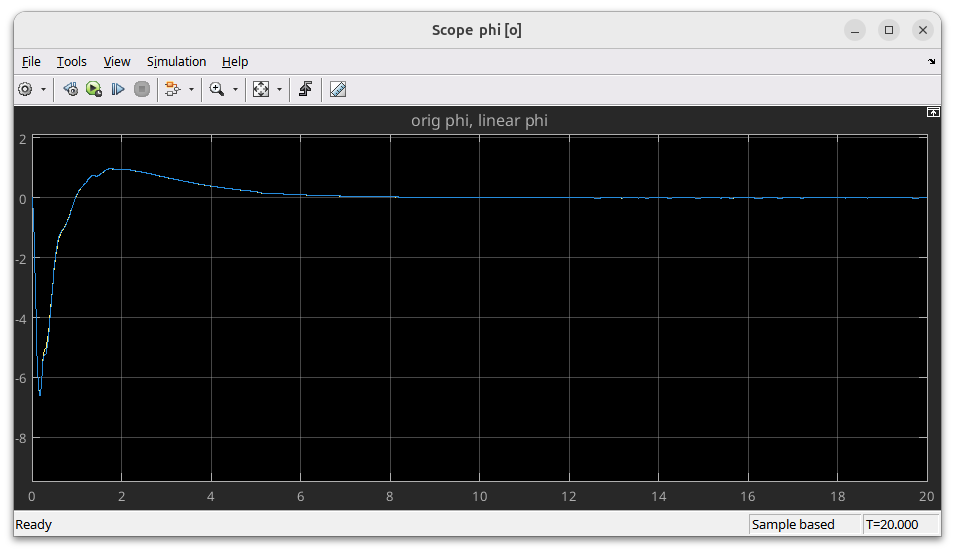
\includegraphics[width=0.8\textwidth]{img/posicast_phi.png}
  \caption{Úhel kyvadla s poisicastem}\label{fig:posicast_phi}
\end{figure}

\section{Řízení pomocí stavové zpětné vazby}
Pomocí stavových metod (moje lineární kyvadlo má 4 stavy - polohu, rychlost,
úhel, úhlovou rychlost) bych chtěl implementovat řízení s kyvadlem nejen v
dolní, ale i v horní poloze. 

\subsection{Řízení pomocí stavové zpětné vazby s předfiltrem}
\subsubsection{Dolní poloha}
Nejdříve vypočítám matici K. Určím (zatím pouze odhadnu) póly na $p = [-3+2i,
-3-2i, -10, -12]$ a matici K dostanu funkcí Matlabu \texttt{place}, která ji
spočítá dle Ackermanova vzorce. Předfiltr vypočítám pomocí vzorce (s
$\mathbf{D}=0$) $\mathbf{M} = \frac{-1}{\mathbf{C}(\mathbf{A} -
\mathbf{BK})\mathbf{B}}$.  Schéma zapojím do Simulinku (obsahuje i regulátor pro
horní polohu), viz obrázek~\ref{fig:state_prefilter_simulink}.

\begin{figure}[htbp]
  \centering
  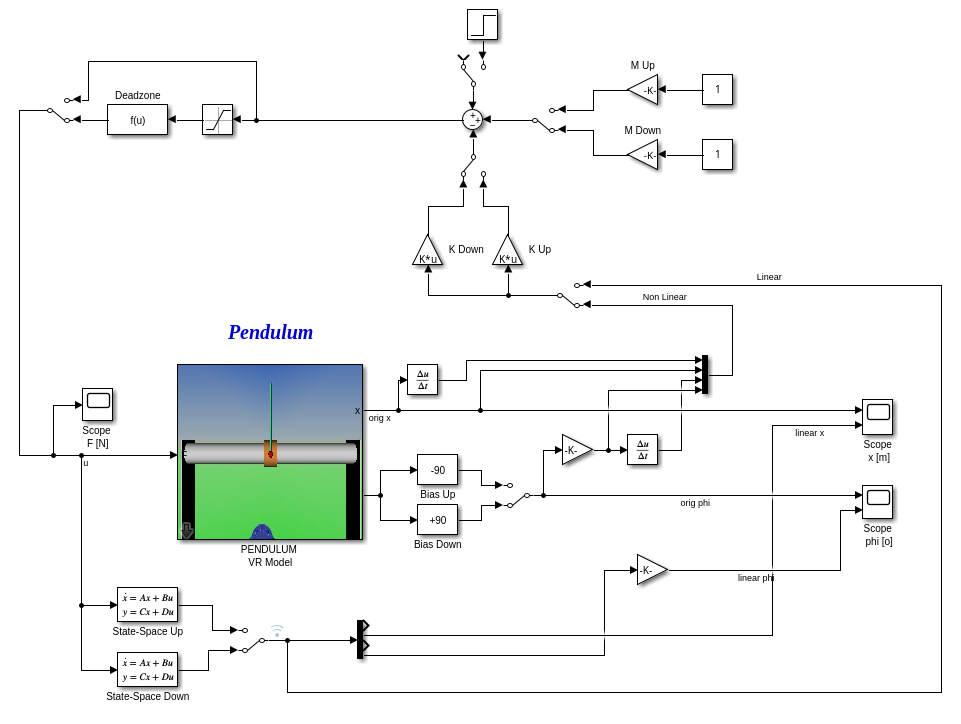
\includegraphics[width=0.8\textwidth]{img/state_prefilter_simulink.png}
  \caption{Zapojení stavové zpětné vazby s předfiltrem v Simulinku}\label{fig:state_prefilter_simulink}
\end{figure}

Z grafu~\ref{fig:state_prefilter_phi_old} vidím, že kyvadlo během pohybu velmi
kmitá. Toto kmitání bych chtěl utlumit, zvolím proto komplexně sdružené póly
tak, aby měly stejnou imaginární hodnotu, jako matice $\mathbf{A}$, ale větší
reálnou hodnotu. Zbylé dva póly zmenším tak, abych vstupním napětím
nedosahoval na saturaci, tedy $p = [-7-13.52i, -7+13.52i, -1.2, -1]$.
Výsledek vidím na obrázcích~\ref{fig:state_prefilter_x}
a~\ref{fig:state_prefilter_phi_new}.

\begin{figure}[htbp]
  \centering
  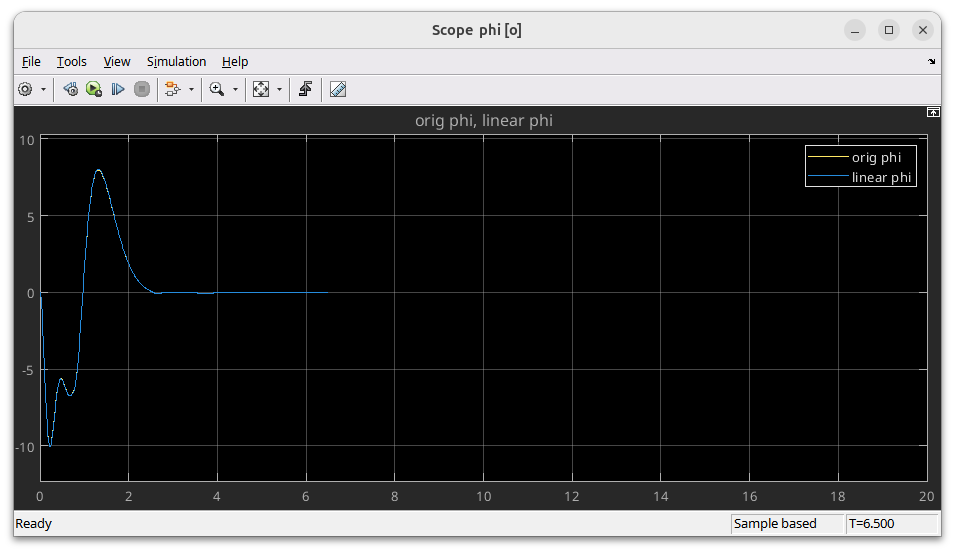
\includegraphics[width=0.8\textwidth]{img/state_prefilter_phi_old.png}
  \caption{Úhel kyvadla s neodladěnými póly}\label{fig:state_prefilter_phi_old}
\end{figure}

\begin{figure}[htbp]
  \centering
  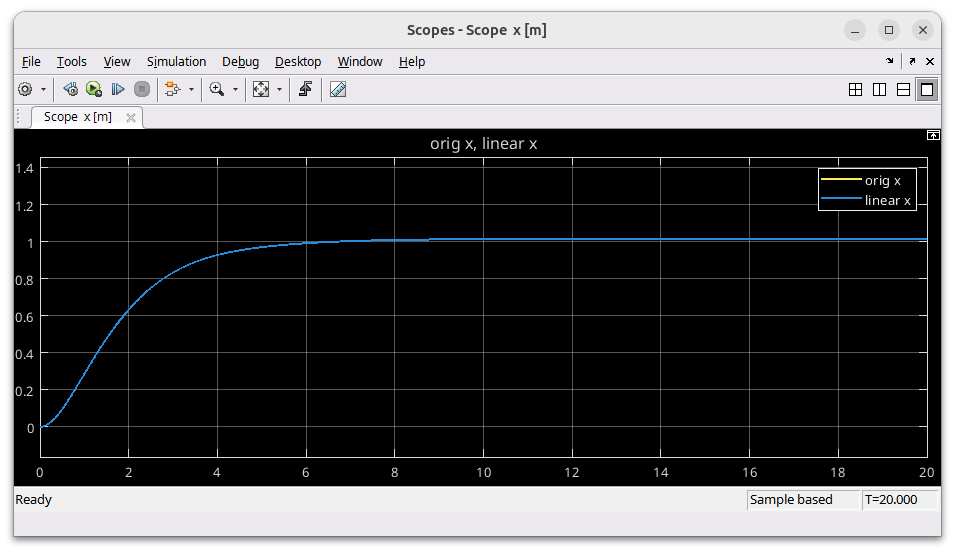
\includegraphics[width=0.8\textwidth]{img/state_prefilter_x.png}
  \caption{Poloha vozíku se stavovou zpětnou vazbou}\label{fig:state_prefilter_x}
\end{figure}

\begin{figure}[htbp]
  \centering
  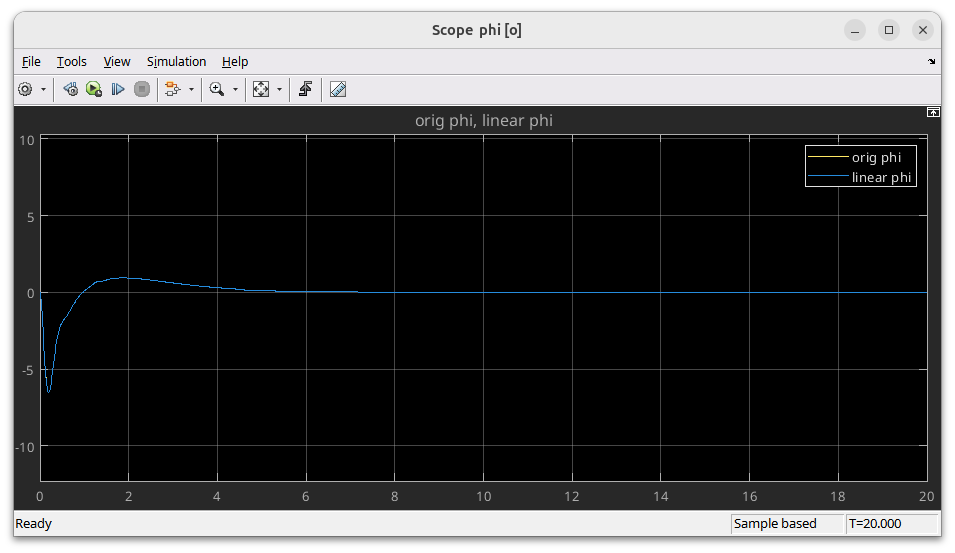
\includegraphics[width=0.8\textwidth]{img/state_prefilter_phi_new.png}
  \caption{Úhel kyvadla se stavovou zpětnou vazbou}\label{fig:state_prefilter_phi_new}
\end{figure}

\subsubsection{Horní poloha}
S póly $p = [-19, -11+3i, -11-3i, -0.25]$ jsem schopen kyvadlo udržet v horní
poloze. Rychlý pól v poloze $-19$ jsem zvolil tak, aby odpovídal pólu kyvadla v
$-18.98$, komplexně sdružené póly vyrovnávají padání kyvadla - jeho nestabilní
pól v bodě $10.56$. Poslední pól jsem volil tak, aby se kyvadlo drželo v horní
poloze s minimální změnou úhlu a zároveň co nejdříve dojelo na stanovenou
pozici. Výsledky jsou na obrázcích~\ref{fig:state_prefilter_up_x}
a~\ref{fig:state_prefilter_up_phi}.

\begin{figure}[htbp]
  \centering
  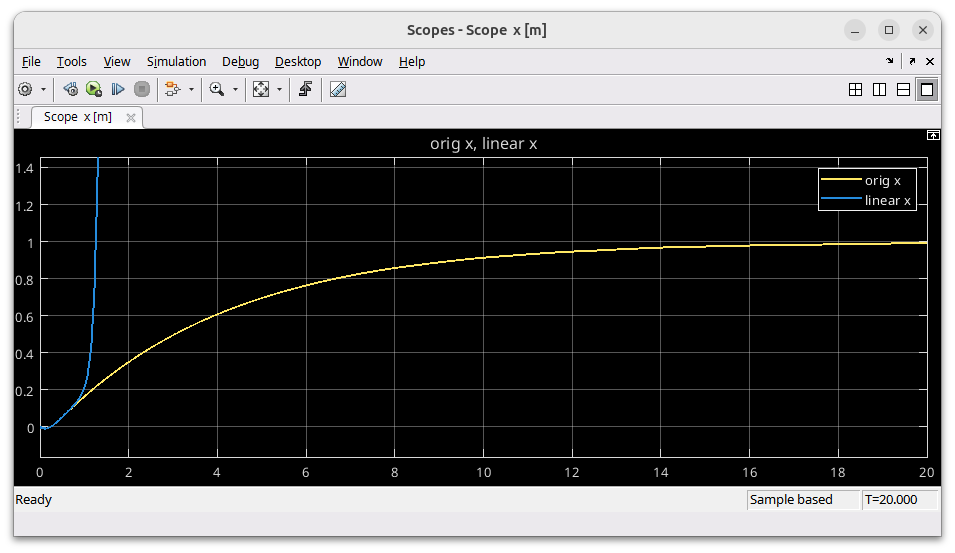
\includegraphics[width=0.8\textwidth]{img/state_prefilter_up_x.png}
  \caption{Stavová zpětná vazba pro horní polohu kyvadla s předfiltrem - poloha}\label{fig:state_prefilter_up_x}
\end{figure}

\begin{figure}[htbp]
  \centering
  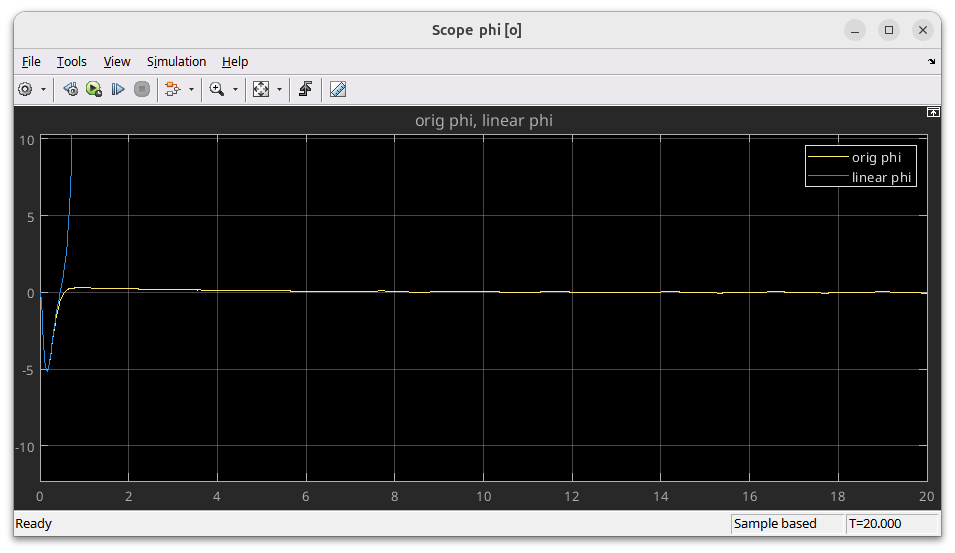
\includegraphics[width=0.8\textwidth]{img/state_prefilter_up_phi.png}
  \caption{Stavová zpětná vazba pro horní polohu kyvadla s předfiltrem - úhel}\label{fig:state_prefilter_up_phi}
\end{figure}


\subsubsection{Problémy implementace s předfiltrem}
Implementace s předfiltrem je ovšem náchylná na poruchy, kvůli kterým vzniká
ustálená odchylka, viz \ref{fig:state_prefilter_x_disorder}, kde jsem přidal
step o hodnotě 1 v čase 2. Proto je potřeba implementovat integrální řízení.

\begin{figure}[htbp]
  \centering
  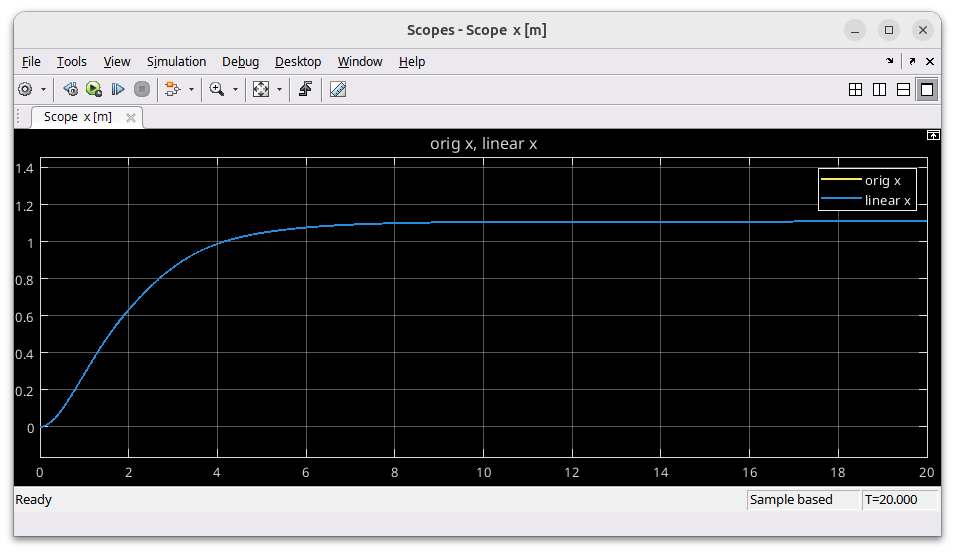
\includegraphics[width=0.8\textwidth]{img/state_prefilter_x_disorder.png}
  \caption{Ustálená odchylka jako reakce na poruchu}\label{fig:state_prefilter_x_disorder}
\end{figure}

\subsection{Integrální řešení stavové zpětné vazby}
Pro integrální řešení odstraním matici $\mathbf{M}$ a místo ní přidám integrátor
za výstup polohy, výslednou zintegrovanou hodnotu vynásobím konstantou $K_i$ a
odečítám od výstupu z matice $\mathbf{K}$. Schéma je na
obrázku~\ref{fig:state_integral_simulink}.

\begin{figure}[htbp]
  \centering
  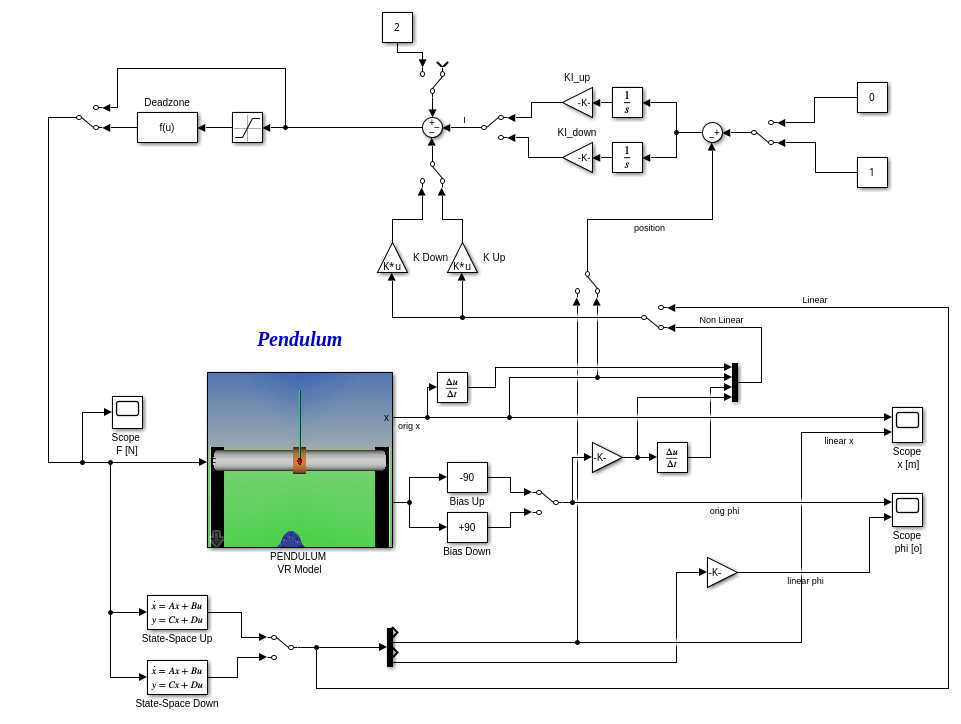
\includegraphics[width=0.8\textwidth]{img/state_integral_simulink.png}
  \caption{Zapojení stavové zpětné vazby s integrálním řešením v Simulinku}\label{fig:state_integral_simulink}
\end{figure}

V Matlabu musím vypočítat hodnotu $K_i$. Nejdříve vytvořím složené matice
$\mathbf{A}$ a $\mathbf{B}$: do matice $\mathbf{A}$ přidám řádek s $-\mathbf{C}
= \begin{bmatrix} 0 & -1 & 0 & 0 \end{bmatrix}$, protože integrální složkou chci
doladit polohu. Zbytek složených matic doplním nulami. Matice $\mathbf{K}$,
kterou opět dostanu funkcí \texttt{place}, bude mít tentokráte $5$ hodnot - tou
pátou bude $K_i$. Póly pro dolní polohu jsem zvolil jako $p = [-7+13.5160i,
-7-13.5160i, -3, -2, -1]$ a pro horní polohu jako $p=[-19, -11+3i, -11-3i, -2,
-0.5]$.

Integrální řešení je odolné i vůči konstantnímu působení síly některým směrem
(mohu si to představit tak, že je rovina s kyvadlem nahnutá z kopce). Následují 
ukázky grafů s působící konstantní silou o hodnotě $2 \mathrm{V}$ pro dolní a horní polohu 
kyvadla.

\begin{figure}[htbp]
  \centering
  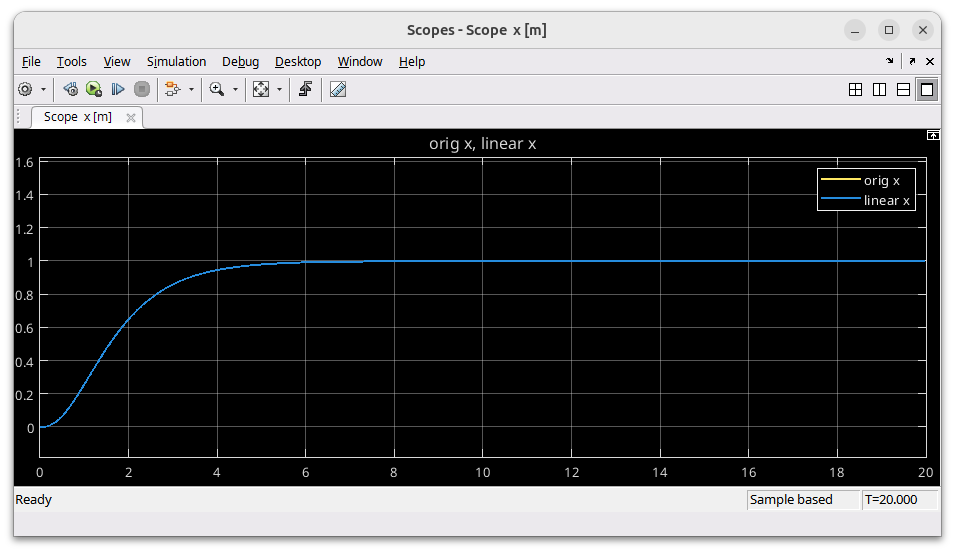
\includegraphics[width=0.8\textwidth]{img/state_integral_down_x.png}
  \caption{Stavová zpětná vazba pro dolní polohu: x}\label{fig:state_integral_down_x}
\end{figure}

\begin{figure}[htbp]
  \centering
  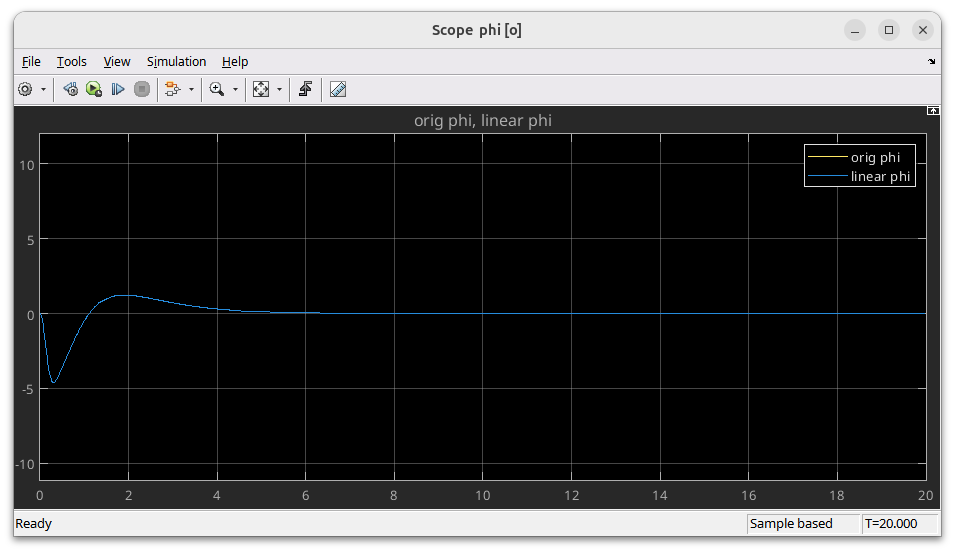
\includegraphics[width=0.8\textwidth]{img/state_integral_down_phi.png}
  \caption{Stavová zpětná vazba pro dolní polohu: $\varphi$}\label{fig:state_integral_down_phi}
\end{figure}

\begin{figure}[htbp]
  \centering
  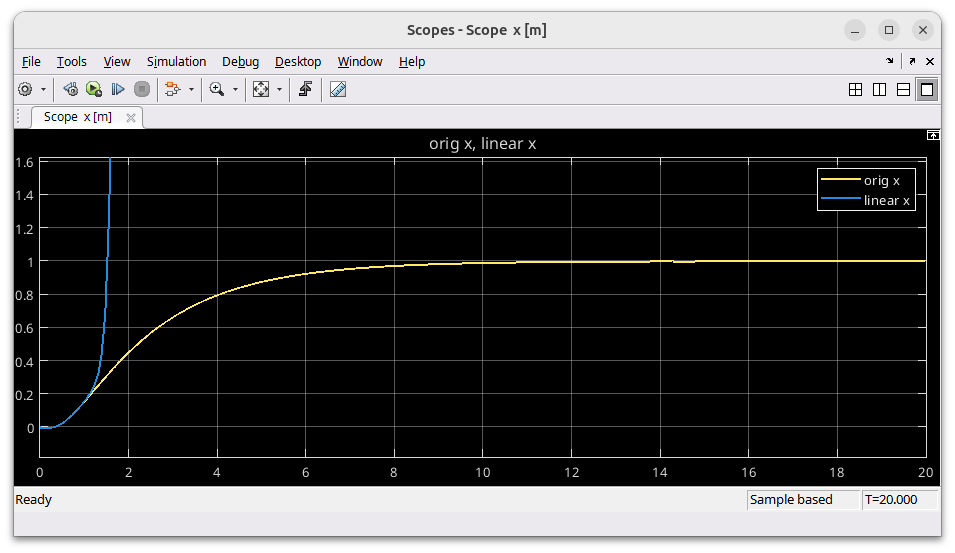
\includegraphics[width=0.8\textwidth]{img/state_integral_up_x.png}
  \caption{Stavová zpětná vazba pro horní polohu: x}\label{fig:state_integral_up_x}
\end{figure}

\begin{figure}[htbp]
  \centering
  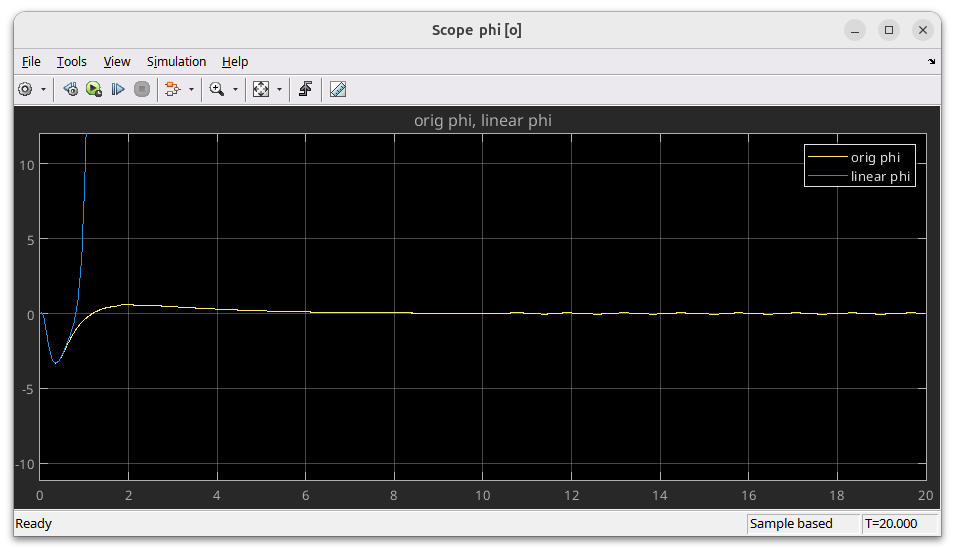
\includegraphics[width=0.8\textwidth]{img/state_integral_up_phi.png}
  \caption{Stavová zpětná vazba pro horní polohu: $\varphi$}\label{fig:state_integral_up_phi}
\end{figure}

\subsection{Pozorovatel}
Obzvláště pro řízení reálného kyvadla je nutné implementovat pozorovatele, který
bude určovat rychlost a úhlovou rychlost kyvadla - ty se totiž neměří senzorem.
Pro pozorovatele na horní i dolní polohu vyberu póly (volil jsem je $\pm2$
krát rychlejší než rychlé póly regulátoru) a v Matlabu spočítám matici $\mathbf{L}$
pomocí \texttt{L = place(A', C', p)'}. Následně zapojím do Simulinku jako na
obrázku~\ref{fig:observer_simulink}.

\begin{figure}[htbp]
  \centering
  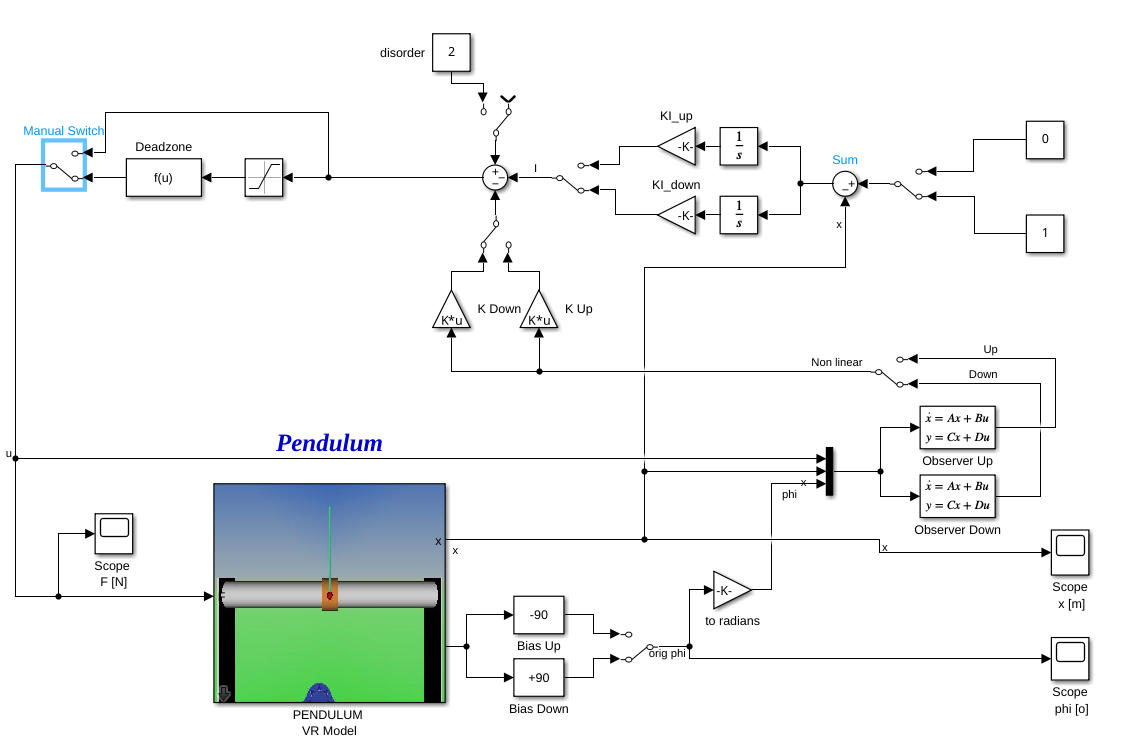
\includegraphics[width=0.8\textwidth]{img/observer_simulink.png}
  \caption{Zapojení pozorovatele v Simulinku}\label{fig:observer_simulink}
\end{figure}

Zapojení pozorovatele jsem otestoval tak, že jsem odpojil zpětnout vazbu, do 
vozíku poslal sinusový signál, nastavil kyvadlo na $-60^\circ$ stupňů namísto
$-90^\circ$ a sledoval, jestli pozorovatel dorovná signál z VR modelu, což se
také stalo, viz obrázek~\ref{fig:observer_test}.

\begin{figure}[htbp]
  \centering
  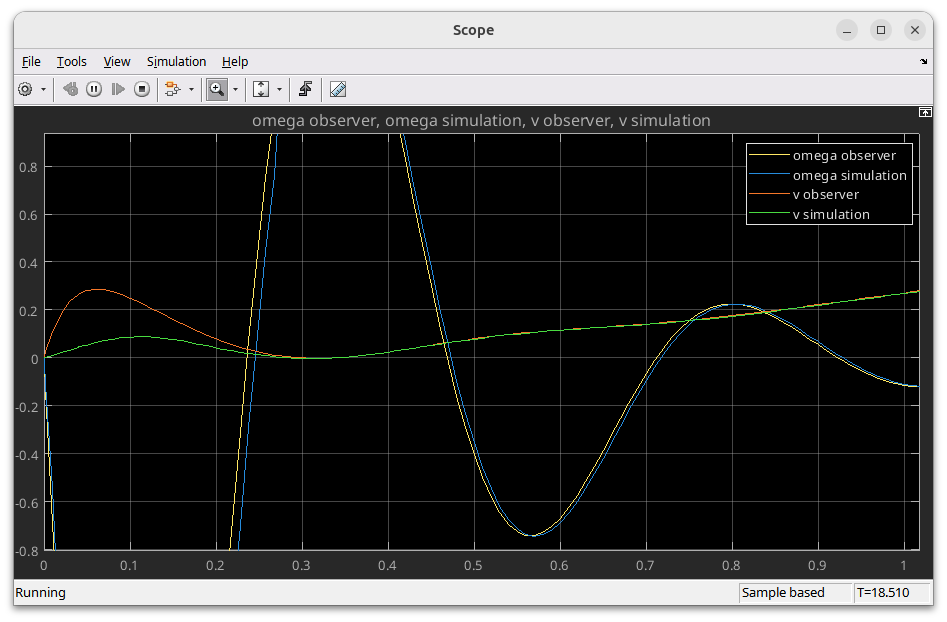
\includegraphics[width=0.8\textwidth]{img/observer_test.png}
  \caption{Testování pozorovatele - graf rychlosti a úhlové rychlosti}\label{fig:observer_test}
\end{figure}

\subsubsection{Rychlejší přechod}
S pozorovatelem vyzkouším ještě volbu pólů pro co nejrychlejší přechod bez
ohledu na kyvadlo, zvolil jsem $p = [-8+13.5i, -8-13.5i, -10, -8, -1]$. Výsledky
jsou na obrázcích~\ref{fig:state_fast_x} a~\ref{fig:state_fast_phi}.

\begin{figure}[htbp]
  \centering
  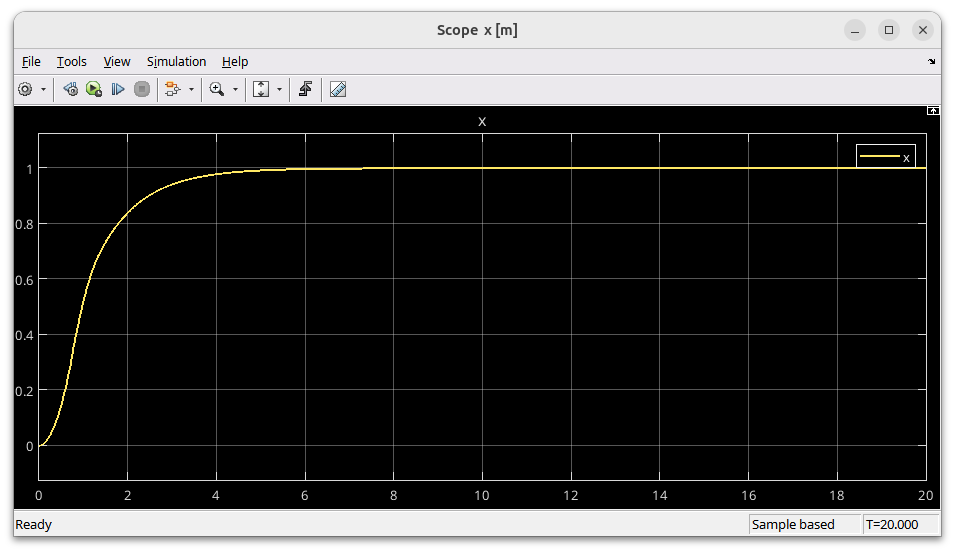
\includegraphics[width=0.8\textwidth]{img/state_fast_x.png}
  \caption{Rychlá regulace na bod 1 - poloha}\label{fig:state_fast_x}
\end{figure}

\begin{figure}[htbp]
  \centering
  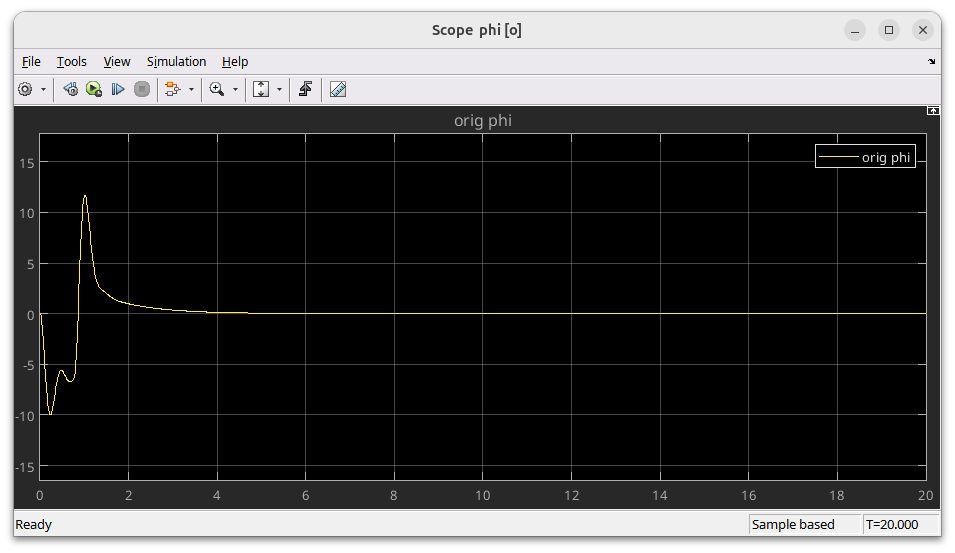
\includegraphics[width=0.8\textwidth]{img/state_fast_phi.png}
  \caption{Rychlá regulace na bod 1 - úhel}\label{fig:state_fast_phi}
\end{figure}

\section{Navazující úloha - práce se skutečným lineárním kyvadlem}
Jako navazující úlohu jsem si vybral řízení lineárního kyvadla, které máme k
dispozici v laboratoři. Práce probíhá podobně jako v simulaci, tedy vytvářím
program skrz Siumulink, který za běhu ovládá reálné kyvadlo a vrací mi polohu a
úhel kyvadla. Oproti simulaci má kyvadlo ovšem jiné vlastnosti, kterým budu
muset přizpůsobit své regulátory.

\subsection{Identifikace systému}
Nejdříve je nutné identifikovat systém. Rozhodl jsem se pro zjištění parametrů
kyvadla, abych dostal nové matice $\mathbf{A}$ a $\mathbf{B}$ a mohl použít
stejné výpočty, jako v simulaci, pouze s novými maticemi. Přípustné hodnoty
vstupního napětí jsou v rozsahu $u \in [-1, 1]$, ale reálné napětí je desetkrát
větší, tedy $u \in [-10, 10] \mathrm{[V]}$. Deadzone jsem postupným zvyšováním
napětí identifikoval přibližně na hodnotu 0.14.

Co se samotných veličin týče, tak délku kyvadla jsem změřil na $l=0.11
\mathrm{m}$ a vzdálenost od konce kyvadla k jeho těžišti na $l_{cm} = 0.04
\mathrm{m}$. Hmotnost kyvadla jsem zvážil kuchyňskou váhou jako $m=0.157
\mathrm{kg}$ a hmotnost vozíku jako $M=0.55 \mathrm{kg}$.

Dále jsem potřeboval zjistit moment hybnosti kyvadla. Zabrzdil jsem vozík
a nechal kyvadlo volně kmitat. Perioda mezi kmity vyšla jako $T=0.58
\mathrm{s}$, z čehož dostávám úhlovou rychlost $\omega=\frac{2\pi}{T} = 10.83
\mathrm{rad} \cdot \mathrm{s}^{-1}$. Moment hybnosti spočítám jako $J =
\frac{m g l_{cm}}{\omega^2} = 5.64\cdot10^{-4} \mathrm{kg}\cdot\mathrm{m}^{-2}$.

Pro konstantu tření vozíku vezmu opět graf, při kterém kyvadlo volně kmitá.
Vyberu si první a pátý kmit, vypočítám logaritmus podílu jejich amplitud a
vydělím $5$: $\Lambda =
\frac{1}{5}\ln\left(\frac{\Lambda_1}{\Lambda_5}\right) =
\frac{1}{5}\ln\left(\frac{1.655}{1.215}\right) = 0.174$

Už mi chybí pouze konstanta tření vozíku a podíl vstupního napětí vůči působící
síle. Pro test odmontuji kyvadlo, aby neovlivňovalo pohyb vozíku. Chci
provést přechodový děj - do vozíku pustím konstantní napětí $U_{in} = 4
\mathrm{V}$ po dobu $1.6 \mathrm{s}$. Zjistím čas $\tau=0.26\mathrm{s}$, za
který vozík dosáhne $63\%$ rychlosti. Konstantu tření vozíku spočítám jako $b
= \frac{M}{\tau} = 2.12$. Podíl vstupního napětí vůči působící síle získám jako
$k_f = b\frac{v_{max}}{U_{in}} = 2.96 \mathrm{N}\cdot \mathrm{V}^{-1}$.

\subsection{PID regulátor polohy s tlumením kmitů}
Schéma zapojení zůstává stejné, jako v simulaci. Získal jsem nové matice 
představující kyvadlo, takže pomocí nástroje \texttt{rltool} odladím
hodnoty regulátoru pro pohyb vozíku a pro tlumení kyvadla. Grafy lze vidět na
obrázcích~\ref{fig:real_rltool_pid_pos} a~\ref{fig:real_rltool_phi}.

\begin{figure}[htbp]
  \centering
  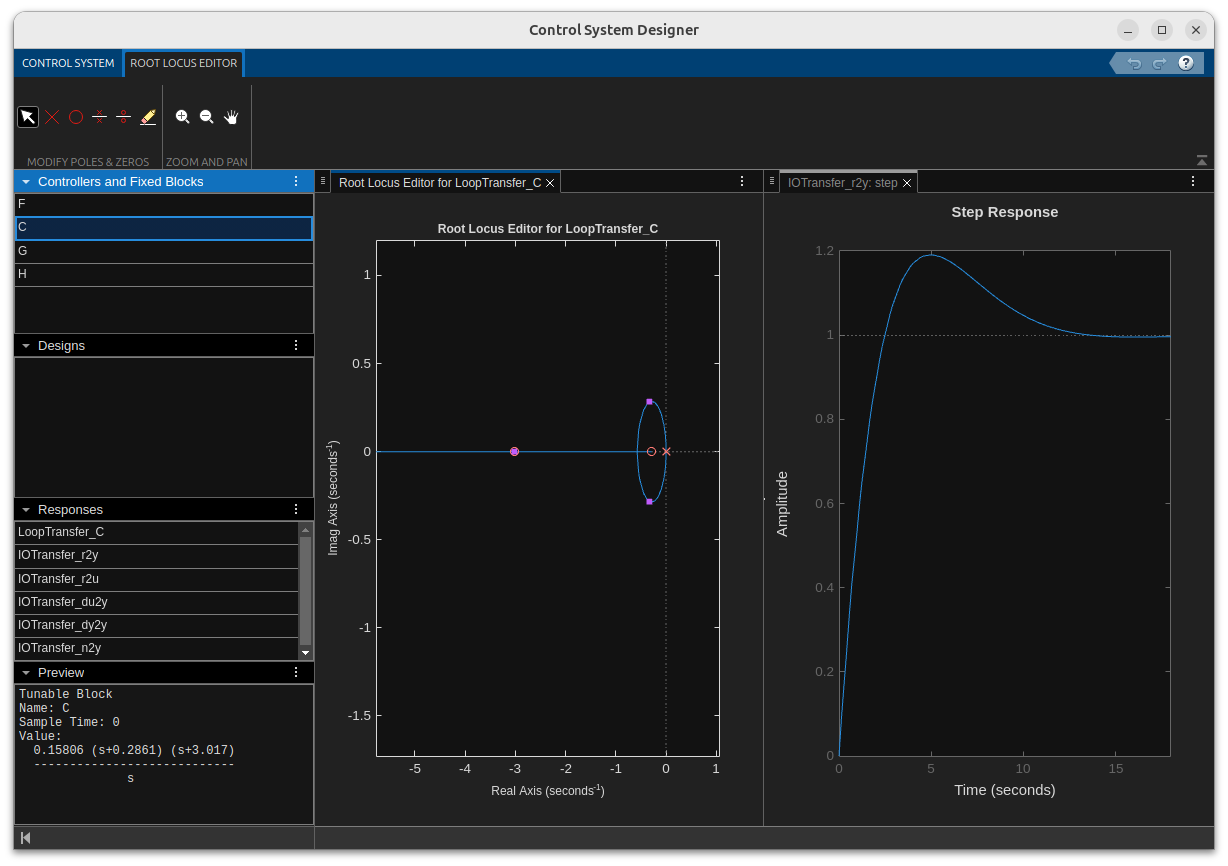
\includegraphics[width=0.8\textwidth]{img/real/rltool_pid_pos.png}
  \caption{Hledání parametrů PID regulátoru pomocí rltool}\label{fig:real_rltool_pid_pos}
\end{figure}

\begin{figure}[htbp]
  \centering
  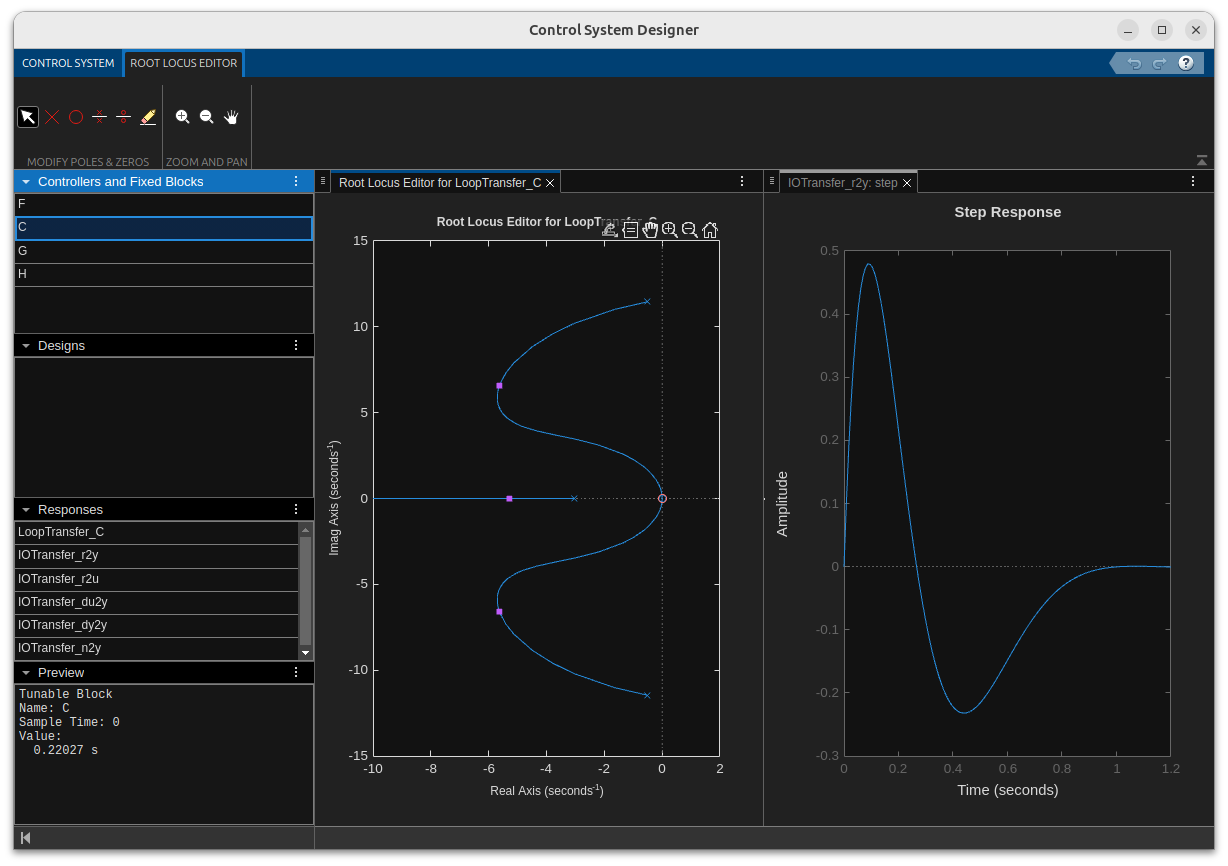
\includegraphics[width=0.8\textwidth]{img/real/rltool_phi.png}
  \caption{Hledání parametrů D regulátoru pomocí rltool}\label{fig:real_rltool_phi}
\end{figure}

Dále uvádím grafy ukazující samotný pohyb kyvadla bez zapnutého tlumení
kmitů~\ref{fig:real_pid_pos_without_d} a s tlumením
kmitů~\ref{fig:real_pid_pos_with_d}.

\begin{figure}[htbp]
  \centering
  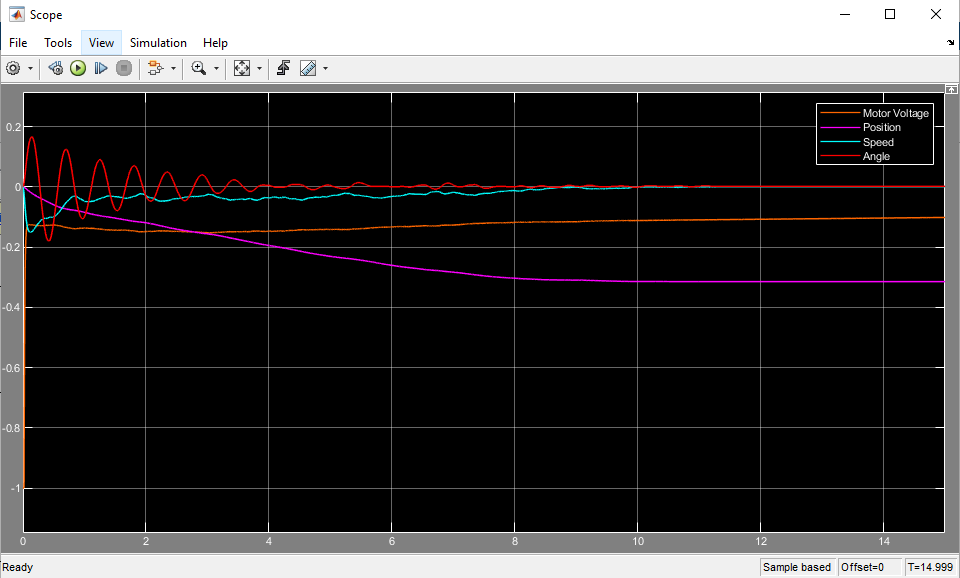
\includegraphics[width=0.8\textwidth]{img/real/pid_pos_without_phi.png}
  \caption{PID regulátor polohy kyvadla bez tlumení kmitů}\label{fig:real_pid_pos_without_d}
\end{figure}

\begin{figure}[htbp]
  \centering
  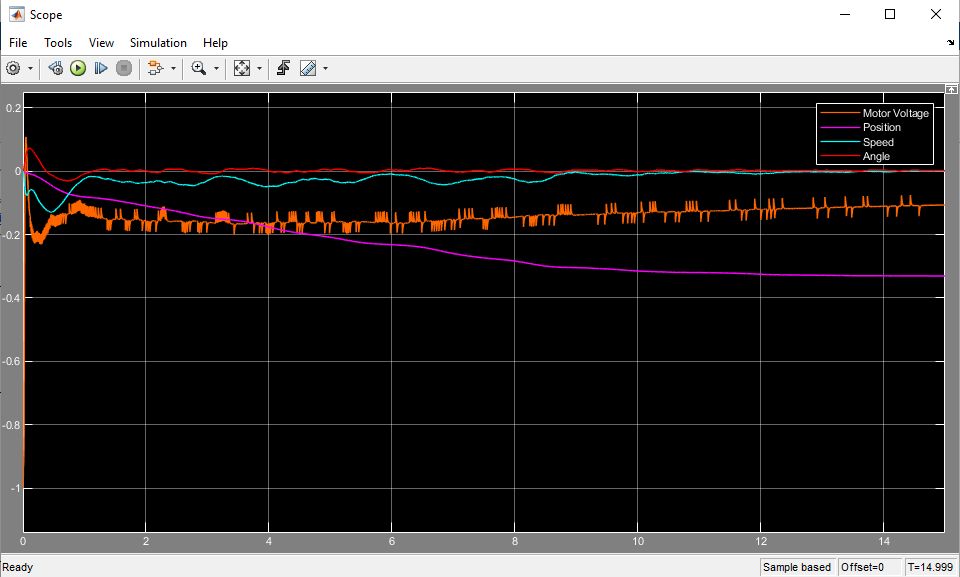
\includegraphics[width=0.8\textwidth]{img/real/pid_pos_with_d.png}
  \caption{PID regulátor polohy kyvadla s tlumením kmitů}\label{fig:real_pid_pos_with_d}
\end{figure}

\subsection{Stavová zpětná vazba}
Pro obě řešení jsem rovnou zvolil metodu s integrálním řešením a s pozorovatelem, protože jsou nejefektivnější.

\subsubsection{Dolní poloha}
Reálné kyvadlo má v dolní poloze následující póly: $0$, $-3.0172$, $-0.5191 \pm
11.4508\,\mathrm{i}$. Stejným postupem jako v simulaci si vyberu následující
póly pro stavové řízení s integrální složkou: $p = [-9+11.4508\mathrm{i}, -9-11.4508\mathrm{i},
-4, -1, -3]$. Výsledný graf pro regulaci na bod $-0.3$ je na
obrázku~\ref{fig:real_state_down}.

\begin{figure}[htbp]
  \centering
  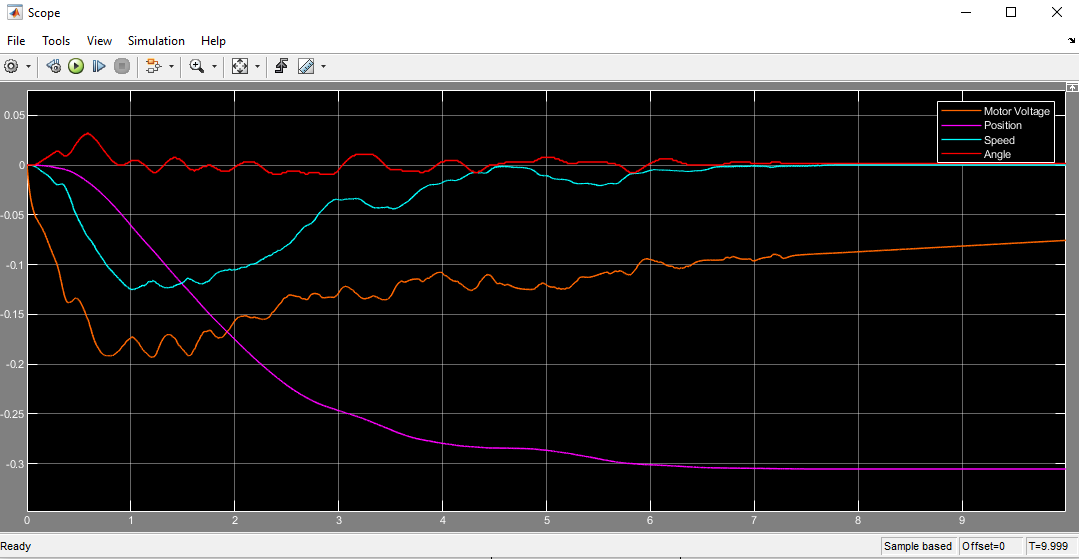
\includegraphics[width=0.8\textwidth]{img/real/state_down.png}
  \caption{Stavová zpětná vazba pro dolní polohu kyvadla}\label{fig:real_state_down}
\end{figure}

\subsubsection{Horní poloha}
Pro horní polohu má kyvadlo následující póly: $0$, $-2.9651$, $-12.1210$,
$11.0306$.  Pro regulátor si vyberu póly $-15$, $-11\pm3i$, $-4$, $-2$. Výsledek
pro řízení kyvadla v horní poloze, když jsem mu jako referenci dával sinusový
signál s amplitudou $0.2$ a frekvenci $0.5 \mathrm{rad}\cdot\mathrm{s}^{-1}$ je
na obrázku~\ref{fig:real_state_up}. Graf pro regulaci v bodě nula, když jsem k
signálu přidával poruchu o velikosti $d = 2 \mathrm{V}$ je na
obrázku~\ref{fig:real_state_up_disorder}.

\begin{figure}[htbp]
  \centering
  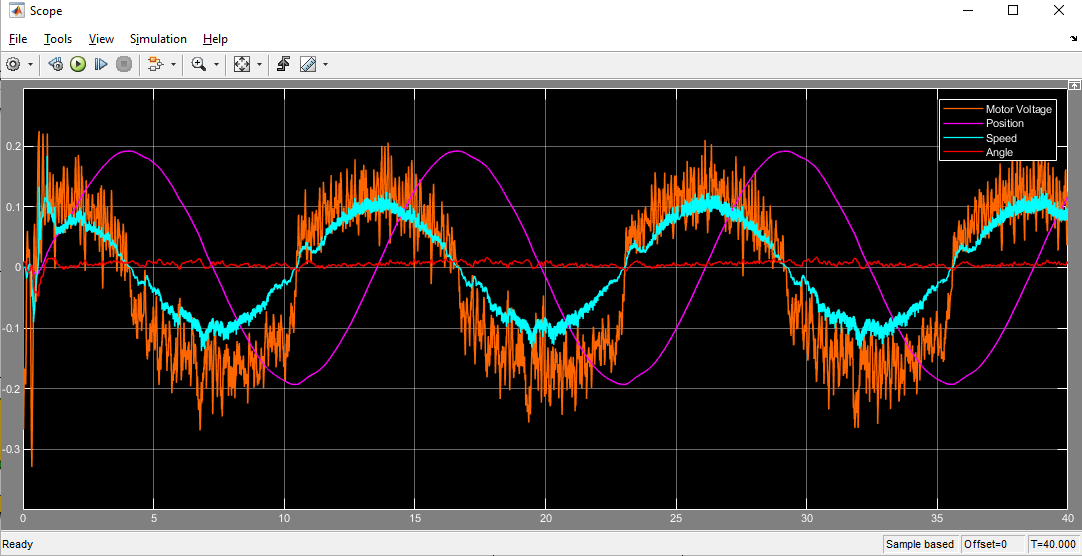
\includegraphics[width=0.8\textwidth]{img/real/state_up.png}
  \caption{Stavová zpětná vazba pro horní polohu kyvadla}\label{fig:real_state_up}
\end{figure}

\begin{figure}[htbp]
  \centering
  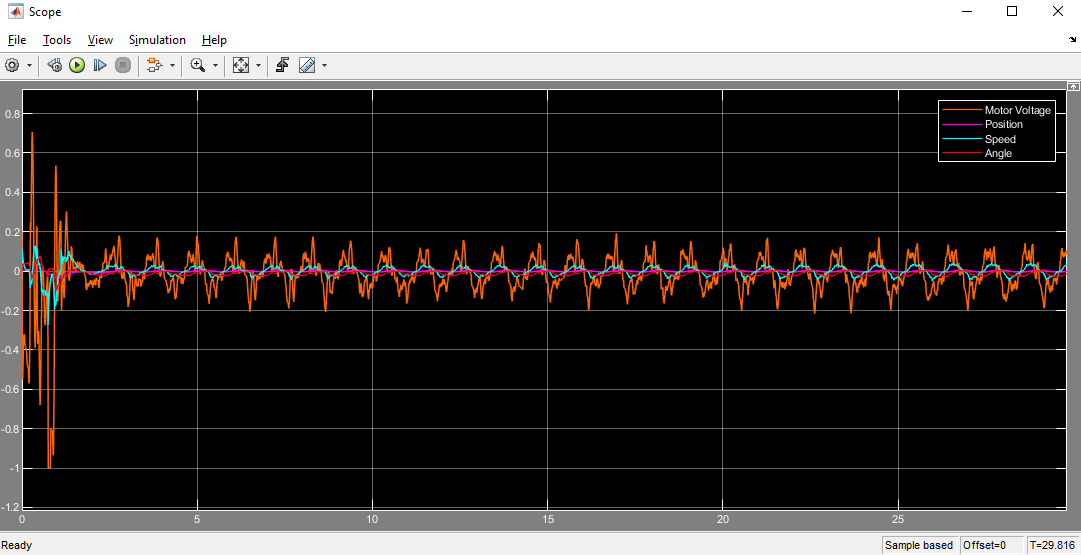
\includegraphics[width=0.8\textwidth]{img/real/state_up_with_disorder.png}
  \caption{Stavová zpětná vazba pro horní polohu kyvadla s poruchu}\label{fig:real_state_up_disorder}
\end{figure}


\begin{thebibliography}{9}
\bibitem{zadani}
Prof. Martin Hromčík. \textit{Inverzni\_kyvadlo\_new.pdf}.
\end{thebibliography}

\end{document}